% Unidad 3
\chapter{Refrigeración por compresión}
\minitoc

	La refrigeración por compresión es el método más utilizado en aplicaciones domésticas, comerciales e industriales para la conservación de alimentos, el aire acondicionado y procesos industriales que requieren temperaturas controladas. Este sistema opera mediante un ciclo termodinámico cerrado, en el que un refrigerante cambia de fase para absorber y ceder calor, permitiendo la transferencia de energía térmica de una zona fría a una más caliente.
	
	El ciclo básico consta de cuatro procesos fundamentales:
	
	\begin{itemize}
		\item Compresión: El refrigerante en estado gaseoso es comprimido, aumentando su presión y temperatura.
		
		\item Condensación: El gas comprimido cede calor al ambiente y se condensa en estado líquido.

		\item Expansión: El líquido refrigerante pasa por una válvula de expansión, reduciendo su presión y temperatura.
		
		\item Evaporación: En el evaporador, el refrigerante absorbe calor del espacio refrigerado y se evapora, repitiendo el ciclo.
	\end{itemize}

%Temas a desarrollar

	\section{Tipos de sistemas de refrigeración por compresión}
	
	Se pueden clasificar según el número de etapas, el tipo de compresor, el método de condensación, y la distribución del refrigerante en el evaporador.
	
	\subsection{Según la distribución del refrigerante en el evaporador}
	
	Los principales tipos de sistemas de refrigeración por compresión clasificados según el tipo de alimentación o distribución del refrigerante en el evaporador son:
	\begin{itemize}
		\item Sistema de expansión directa.
		\item Sistema inundado o de refrigeración por líquido inundado.
		\item \ver{Lo que sigue hay que buscarlo en algún libro o algún lugar más verídico que chatgpt}
		\item Sistema de expansión seca. Caso particular de la expansión directa.
		\item Sistema de película descendente
		\item Sistema de circulación forzada.
		\item Sistema con recirculación por bombeo.
	\end{itemize}
	
	\section{Ciclo de refrigeración por compresión}

\subsection{Elementos fundamentales}

Los sistemas de refrigeranción por compresión constan, básicamente, de cuatro elementos que consideramos fundamentales a través de los cuales circula un fluido refrigerante.

Estos elementos son:

\begin{enumerate}
	\item Compresor
	\item Condensador
	\item Dispositivo de expansión
	\item Evaporador
\end{enumerate}

\begin{figure}[h]
	\centering
	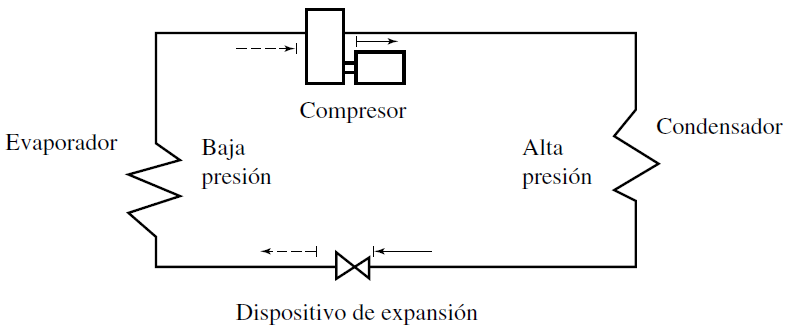
\includegraphics[width=\textwidth]{figuras/elementos fundamentales.png}
	\caption{Elementos fundamentales de un sistema de refrigeración}
	\label{fig:elementos_fundamentales}
\end{figure}


\subsubsection{Funciones principales}

La función de cada uno de ellos es la siguiente:

\textbf{Compresor:}

Aspira el fluido refrigerante a la presión de baja establecida y lo comprime elevando su presión y temperatura hasta unos valores tales que se pueda efectuar la condensación. La descarga la efectua en el condensador.

\textbf{Condensador:}

Es el elemento de la instalación que se encarga de pasar el estado de vapor del fluido refrigerante a estado líquido. El fluido refrigerante entra en el condensador en estado de gas (vapor recalentado) y sale en estado líquido a la temperatura que se condensó o incluso a una temperatura menor si se produce subenfriamiento.

\textbf{Dispositivo de expansión:}

Hace que el fluido, que entra en estado líquido, sufra una caída de presión (y temperatura) hasta la necesaria en el evaporador. También controla la cantidad de fluido refrigerante que debe entrar en el evaporador.

\textbf{Evaporador:}

Se encarga de enfriar o acondicionar la cámara. Puede estar dentro o fuera de la misma. Su misión es que el fluido refrigerante, que entra a baja presión y temperatura, efectúe el enfriamiento.\\
Es el elemento de la instalación donde el fluido refrigerante se evapora, tomando calor del exterior del evaporador debido a la diferencia de temperaturas.

\subsubsection{Fluido refrigerante}

El fluido refrigerante está sometido a cambios de estado a lo largo del circuito:

\begin{itemize}
	\item En el compresor entra en estado de gas, a baja presión y temperatura, y sale con presión y temperatura más altas (recalentado), que es como entra en el condensador.
	\item Del condensador sale estado líquido y entra dispositivo de expansión.
	\item Del dispositivo de expansión sale en forma de mezcla de líquido y gas (expansión), a baja presión y temperatura, y entra en el evaporador.
	\item Del evaporador sale en estado de gas, a baja presión y temperatura, de donde es aspirado por el compresor, y se inicia el nuevo ciclo.
\end{itemize}

Como sabemos, \textit{al aumentar la presión de un fluido se eleva su punto de ebullición, y al disminuir la presión, también disminuye su punto de ebullición.} Esta es una de las claves de la refrigeración.

\subsection{Alta y baja presión}

Debemos diferenciar la parte del circuito que está sometida a una presión alta y la que se encuentra a baja presión (\autoref{fig:elementos_fundamentales}).

\textit{La parte correspondiente a la alta presión está comprendida entre la descarga del compresor y la entrada del dispositivo de expansión.}

Hay que resaltar que la temperatura del fluido refrigerante no es la misma en todo ese tramo:

\begin{itemize}
	\item Entre la salida del compresor y la entrada del condensor el fluido está en estado de gas (gas recalentado).
	\item Se condensa a una temperatura menor y s desde el vale del condensador a esa misma temperatura o menor si se subenfría, con lo cual, la temperaturadel fluido a la entrada del dispositivo de expansión puede ser igual o menor que la de condensación.
\end{itemize}

\textit{La parte que corresponde a la baja presión, es la comprendida entre la salida del dispositivo de expansión y la entrada del compresor.}

La instalación dispone del manoómetro de baja presión para conocer su valor en cada momento. En este tramo, también la temperatura varía (aumenta) desde el evaporador hasta la entrada del compresor.

\subsection{Elementos de seguridad y control}

La \autoref{fig:elementos_seguridad_y_control} representa los cuatro elementos fundamentales para el estudio de sus principales características a los que se añaden los elementos de seguridad y control.

\begin{figure}[H]
	\centering
	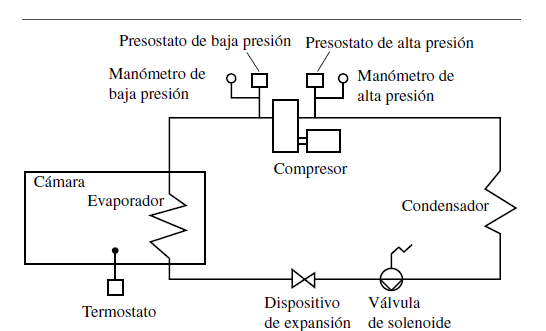
\includegraphics[width=\textwidth]{Elementos_seguridad_y_control.png}
	\caption{Elementos fundamentales de un circuito frigorífico en los que se añaden los dispositivos de seguridad y control.}
	\label{fig:elementos_seguridad_y_control}
\end{figure}

\subsubsection{Presostatos}

Son unos aparatos que, activados por presión, tienen la función de abrir o cerrar un circuito mediante uno o varios contactos normalmente ya sean abiertos o cerrados. De manera práctica, se puede decir que son unos interruptores eléctricos que funcionan por presión. Pueden ser:

\begin{enumerate}
	[a.]
	\item Presostatos de alta presión 
	
	Se conecten a la descarga del compresor, y su función es impedir que en la zona de alta presión, se alcancen valores que afecten al rendimiento de la instalación o a la propia seguridad de las personas. Se regulan a una determinada presión, y cuando la instalación alcanza ese valor, entonces el presostato para el compresor.
	\item Presostatos de baja presión
	
	Se conectan a la aspiración del compresor, y función es evitar que la presión, en la zona baja, pueda ``caer'' por debajo de la presión atmosférica y evitar también que la presión descienda por debajo de la normal de funcionamiento, ya que afectaría al rendimiento. De hecho, su regulación debe estar \textit{siempre} por encima de la presión atmosférica. Cuando la presión descienda hasta la correspondiente al valor de regulación, el presostato parará el compresor. 
\end{enumerate}

Los presostatos de alta y baja presión no tienen que instalarse necesariamente por separado, ya que también se puede instalar los dos formando un solo elemento, llamado \textit{presostato combinado}, tal como se representa en la \autoref{fig:Presostato combinado}.

\begin{figure}[H]
	\centering
	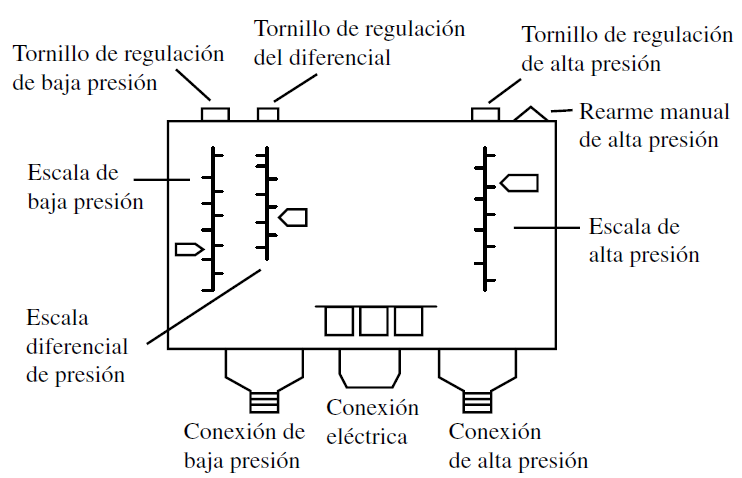
\includegraphics[width=\textwidth]{figuras/presostato combinado.png}
	\caption{Presostato combinado}
	\label{fig:Presostato combinado}
\end{figure}

\subsubsection{Termostato}

Es el elemento que controla la temperatura de la cámara. Abre o cierra un contacto conectado a un circuito eléctrico cuando alcanza la temperatura de regulación. Se puede decir que es un interruptor o conmutador eléctrico que funciona por temperatura.

El termostato con depósito de gas, se basa en que éste sufre variaciones de presión en relación a la temperatura que rodea al depósito que lo contiene. Si una de las paredes del depósitoes de membrana, sufrirá deformaciones a consecuencia de esos cambios de temperatura. Si además actúa sobre unos contactos, bien sea directa o inderectamente, los abrirá o cerrará de acuerdo a la regulación establecida. 

Como los presostatos, disponen de un diferencial (diferencia entre las temperaturas de arranque y de paro) que puede ser fijo o variable. Por lo general suele ser de $\pm 3$.

\textbf{Ejemplo de aplicación}

Queremos mantener una temperatura de -20 \textcelsius en la cámara y el diferencial establecido es de $\pm 3$ \textcelsius.

Ello quiere decir que la instalción se parará cuando la temperatura alcance los -23 \textcelsius, pues el termostato, en ese momento, cerrará la válvula de solenoide. Debido a la transmisión de calor, la temperatura en el interior de la cámara aumentará hasta alcanzar los -17 \textcelsius y entonces el termostato abrirá la válvula de la solenoide, y se pondrá de nuevo en funcionamiento el compresor.

\subsubsection{Válvula de solenoide (o electroválvula)}

Aunque no es un elemento de regulación ni de control, debemos comentar sus principales características para poder enterder mejor el siguiente apartado.

Su funcionamiento es de todo o nada, no es de regulación proporcional. Cuando está activada por el campo magnético, levanta el vástago de la válvula y deja pasar el fluido. Cuando se desactiva, cesa la imanación (no hay campo magnético), el vástago de la válvula cae y corta el paso del fluido refrigerante.

Va conectada en serie con el termostato, por decirlo de una mnera práctica; el termostato deja pasar o corta la corriente eléctrica a la bobina, con lo cual la válvula se abre o cierra, según las necesidades térmicas.


\begin{figure}[H]
	\centering
	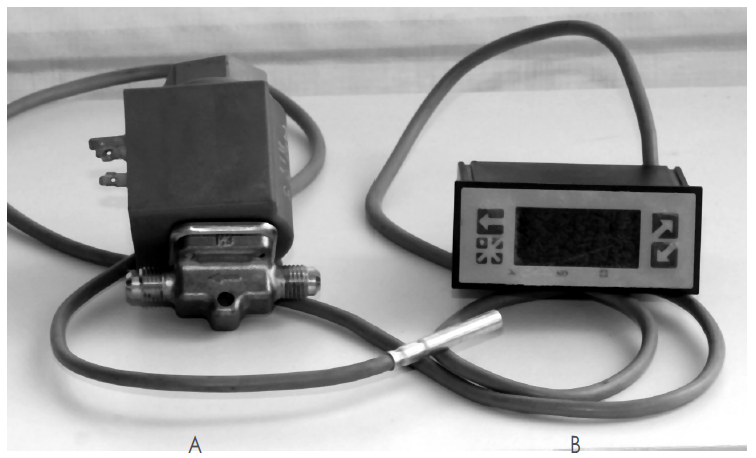
\includegraphics[width=\textwidth]{figuras/solenoide y termometro.png}
	\caption{A: Válvula de solenoide. B:Termostato electrónico}
	\label{fig:solenoide y termostato}
\end{figure}

\subsubsection{Presostato diferencial de aceite}

Es un elemento de seguridad; de hecho es un interruptor de seguridad (\autoref{fig:Presostato diferencial de aceite}). PRotege al compresor contra una presión de aceite demasiado baja. Se conecta a la aspiración y a la descarga de la bomba de lubricación.

\begin{figure}[H]
	\centering
	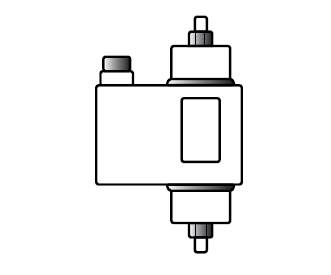
\includegraphics[width=6cm, height=6cm]{figuras/Presostato diferencial de aceite.png}
	\caption{Presostato diferencial de aceite}
	\label{fig:Presostato diferencial de aceite}
\end{figure}

\subsection{Elementos complementarios}
Una instalación podría trabajar con los elementos anteriormente citados, pero, evidentemente, necesita de otros elementos complementarios para que el ciclo de trabajo se pueda efectuar con el mayor rendimiento posible. 

En el siguiente esquema (\autoref{fig:Instalacion con elementos complementarios} se representan los más importantes y su disposición en las instalaciones.)

\begin{figure}[H]
	\centering
	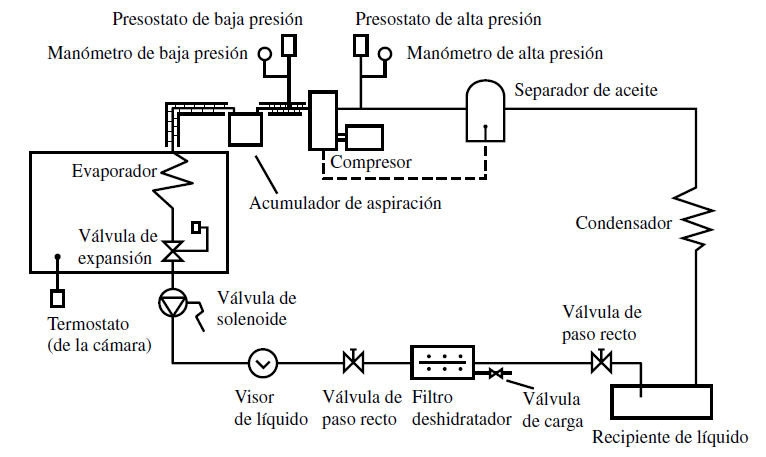
\includegraphics[width=\textwidth]{figuras/Instalación con elementos complementarios.png}
	\caption{Instalación de los elementos fundamentales, de seguridad y control, y complementarios}
	\label{fig:Instalacion con elementos complementarios}
\end{figure}

\subsubsection{Resistencia calefactora (del cárter)}

Cuando las temperaturas que rodean al compresor (temperatura ambiente) son muy bajas, en los tiempos de parada del compresor puede ocurrir que el fluido refrigerante depositado en el cárter se condense, por lo que en el momento del arranque se produce una vaporización rápida del fluido que conlleva un arrastre de aceite.

También la baja temperatura ambiente afecta a la viscosidad del aceite, ya que si es muy baja, ésta aumenta las resistencias a vencer en el arranque. Para evitar estas circunstancias se instalan en el cárter unas peque\~{n}a resistencias eléctricas que lo mantienen a cierta temperatura, de tal manera que cuando para el compresor, entran en funcionamiento.

\subsubsection{Separador de aceite}

Se instala en la tubería de descarga, después del compresor. El fluido refrigerante sale del compresor mezclado con el aceite de lubricación y éste debe retornar al cárter principalmente por dos razones:

\begin{enumerate}
	[1.]
	\item  porque el nivel de aceite del cárter iría disminuyendo y
	\item porque el aceite, cuando llegue al circuito de baja presión, podría tener problemas de retorno (deja de ser miscible y crea problemas en los evaporadores, por ejemplo de transmisión o taponamientos)
\end{enumerate}

Los hay de varios tipos. Por ejemplo los que aprovechan la fuerza centrífuga de la descarga del compresor para efectuar la separación (Figura \ref{fig:Separador de aceite}) o bien la caída de velocidad a la entrada del separador para efectuar la separación.

%     LO DEJO COMENTADO PORQUE DESP TE LO QUIERO MOSTRAR A VER SI VOS SABES QUE PASA
%	Si recortamos las imágenes como para que quede centrado el objeto, mejor :)
\begin{wrapfigure}{r}{0.4\linewidth}
	\centering
	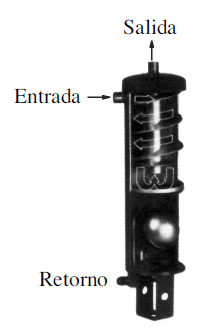
\includegraphics[width=.5\linewidth]{figuras/separador de aceite.png}
	\caption{Separador de aceite}
	\label{fig:Separador de aceite}
\end{wrapfigure}  

El aceite se va decantando en el fondo del separador hasta alcanzar un nivel tal que el regulador, por ejemplo un flotador de nivel, lo detecta y abre el paso de retorno hacia el cárter.

Una representación del retorno de aceite se puede observar en la \autoref{fig:Línea de retorno de aceite}.


Cuando el nivel de aceite en el interior del separador alcanza el nivel estipulado, el regulador de nivel abre la electroválvula y el aceite retorna al cárter. El aceite retorna porque la presión en el interior del separador (presión de alta) es superior a la presión reinante en el cárter.

No tienen una eficacia del 100\%, pero es bueno que una pequeña cantidad de aceite circule por la instalación ya que mantiene engrasados elementos como válvulas, electroválvulas, etc.

\begin{figure}[h]
	\centering
	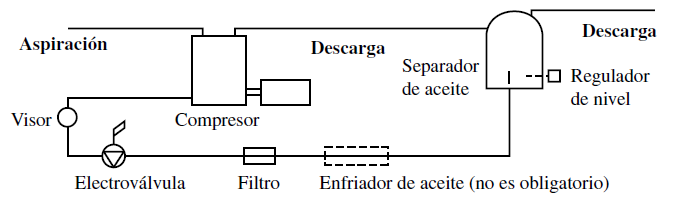
\includegraphics[width=.9\linewidth]{figuras/Linea de retorno de aceite.png}
	\caption{Línea de retorno de aceite}
	\label{fig:Línea de retorno de aceite}
\end{figure}

\subsubsection{Recipiente de líquido}

Se coloca a la salida del condensador, aunque los hay del tipo condensador-recipiente que forman un solo elemento.

El líquido que sale del condensador no va directamente al evaporador, salvo si se utilizan tubos capolares, sino que se ``almacena'' en el recipiente. Mantiene una reserva de líquido para restituirlo según la demanda. Los hay horizontales (\autoref{fig:Recipiente de líquido horizontal}) y (\autoref{fig:Recipiente de líquido vertical}) verticales.

Su capacidad varía con las características de la instalación; si se trata de una con varios evaporadores, su capacidad será por lo menos 1,25 veces la capacidad del evaporador mayor.

\begin{figure}[H]
	\centering
	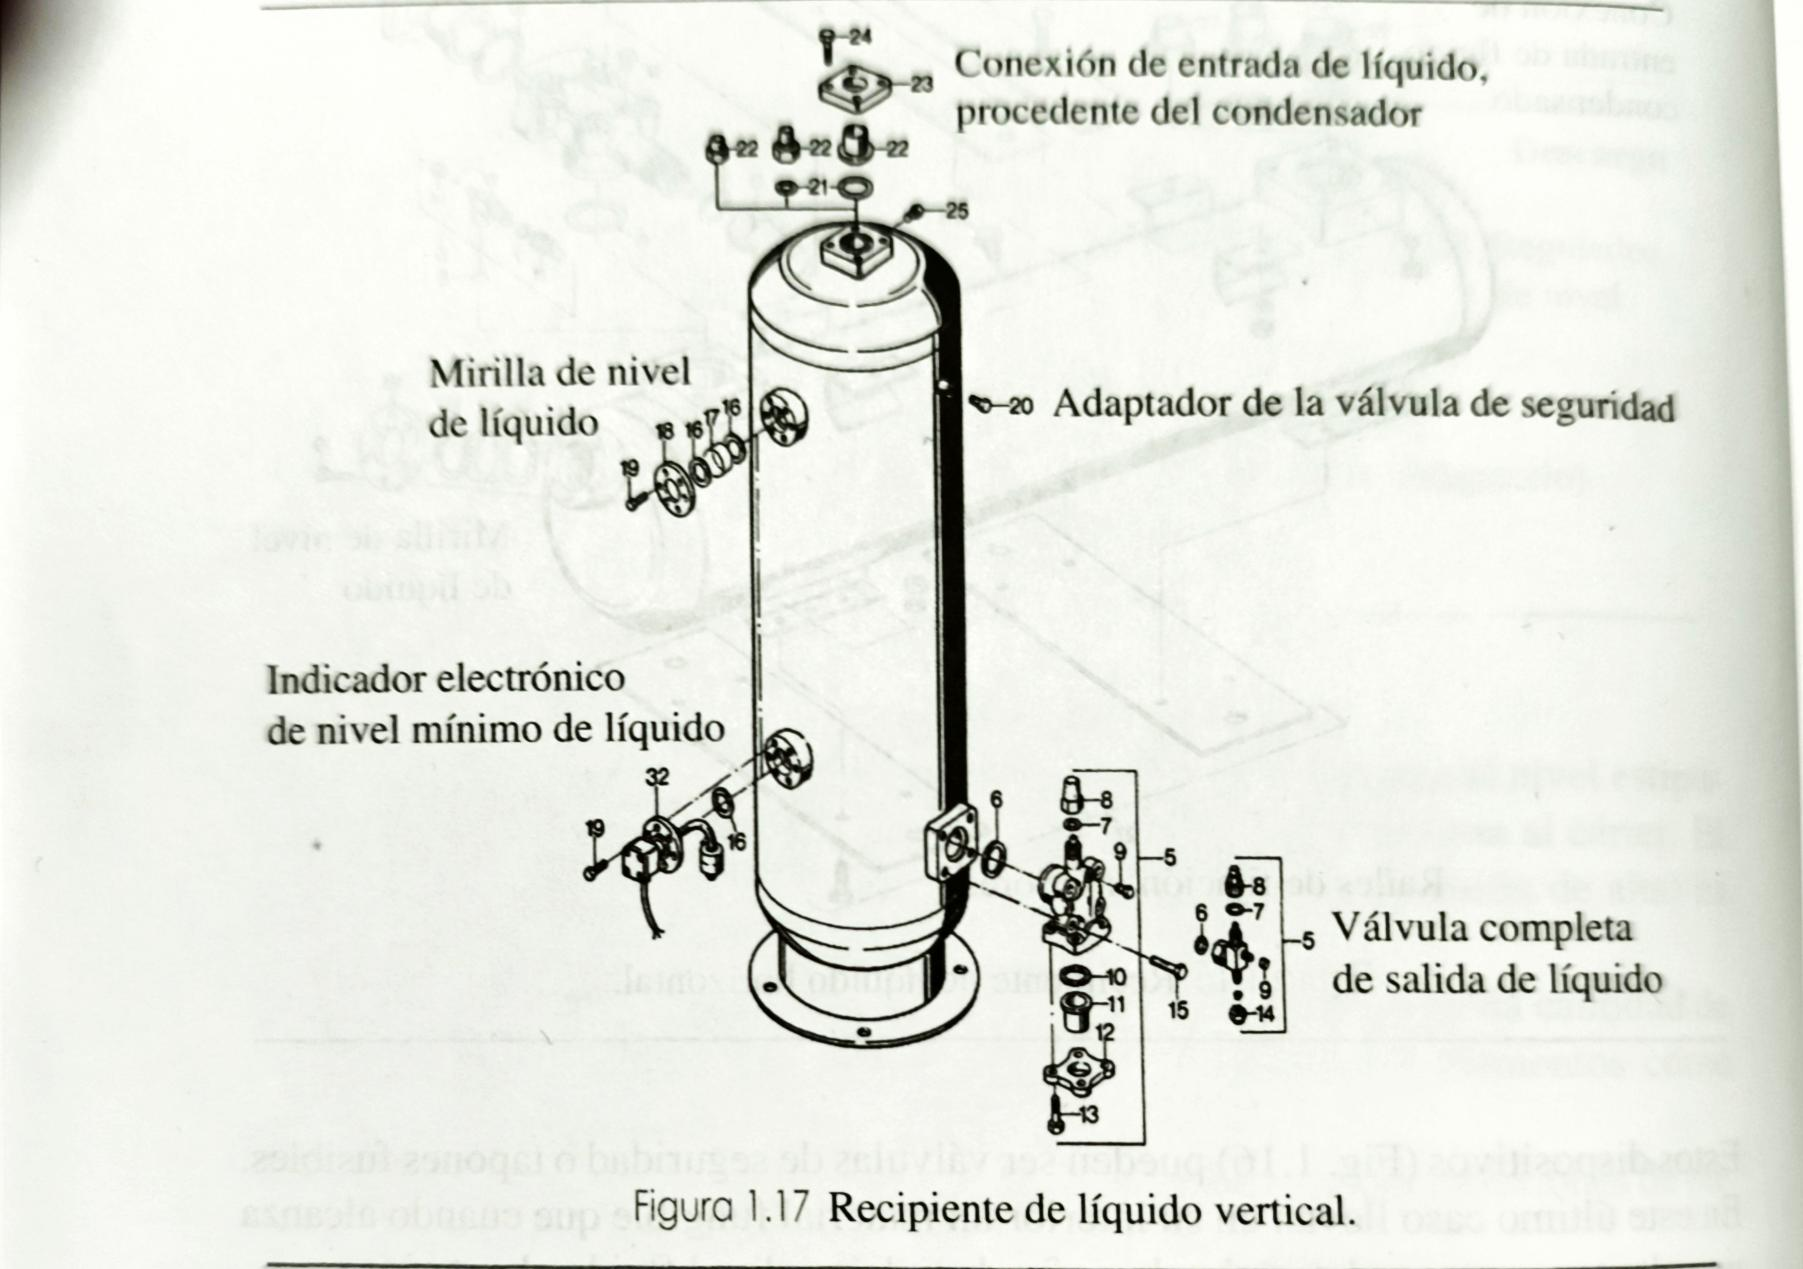
\includegraphics[width=0.7\textwidth]{figuras/recipiente vertical.jpg}
	\caption{Recipiente de líquido vertical}
	\label{fig:Recipiente de líquido vertical}
\end{figure}

\begin{figure}[H]
	\centering
	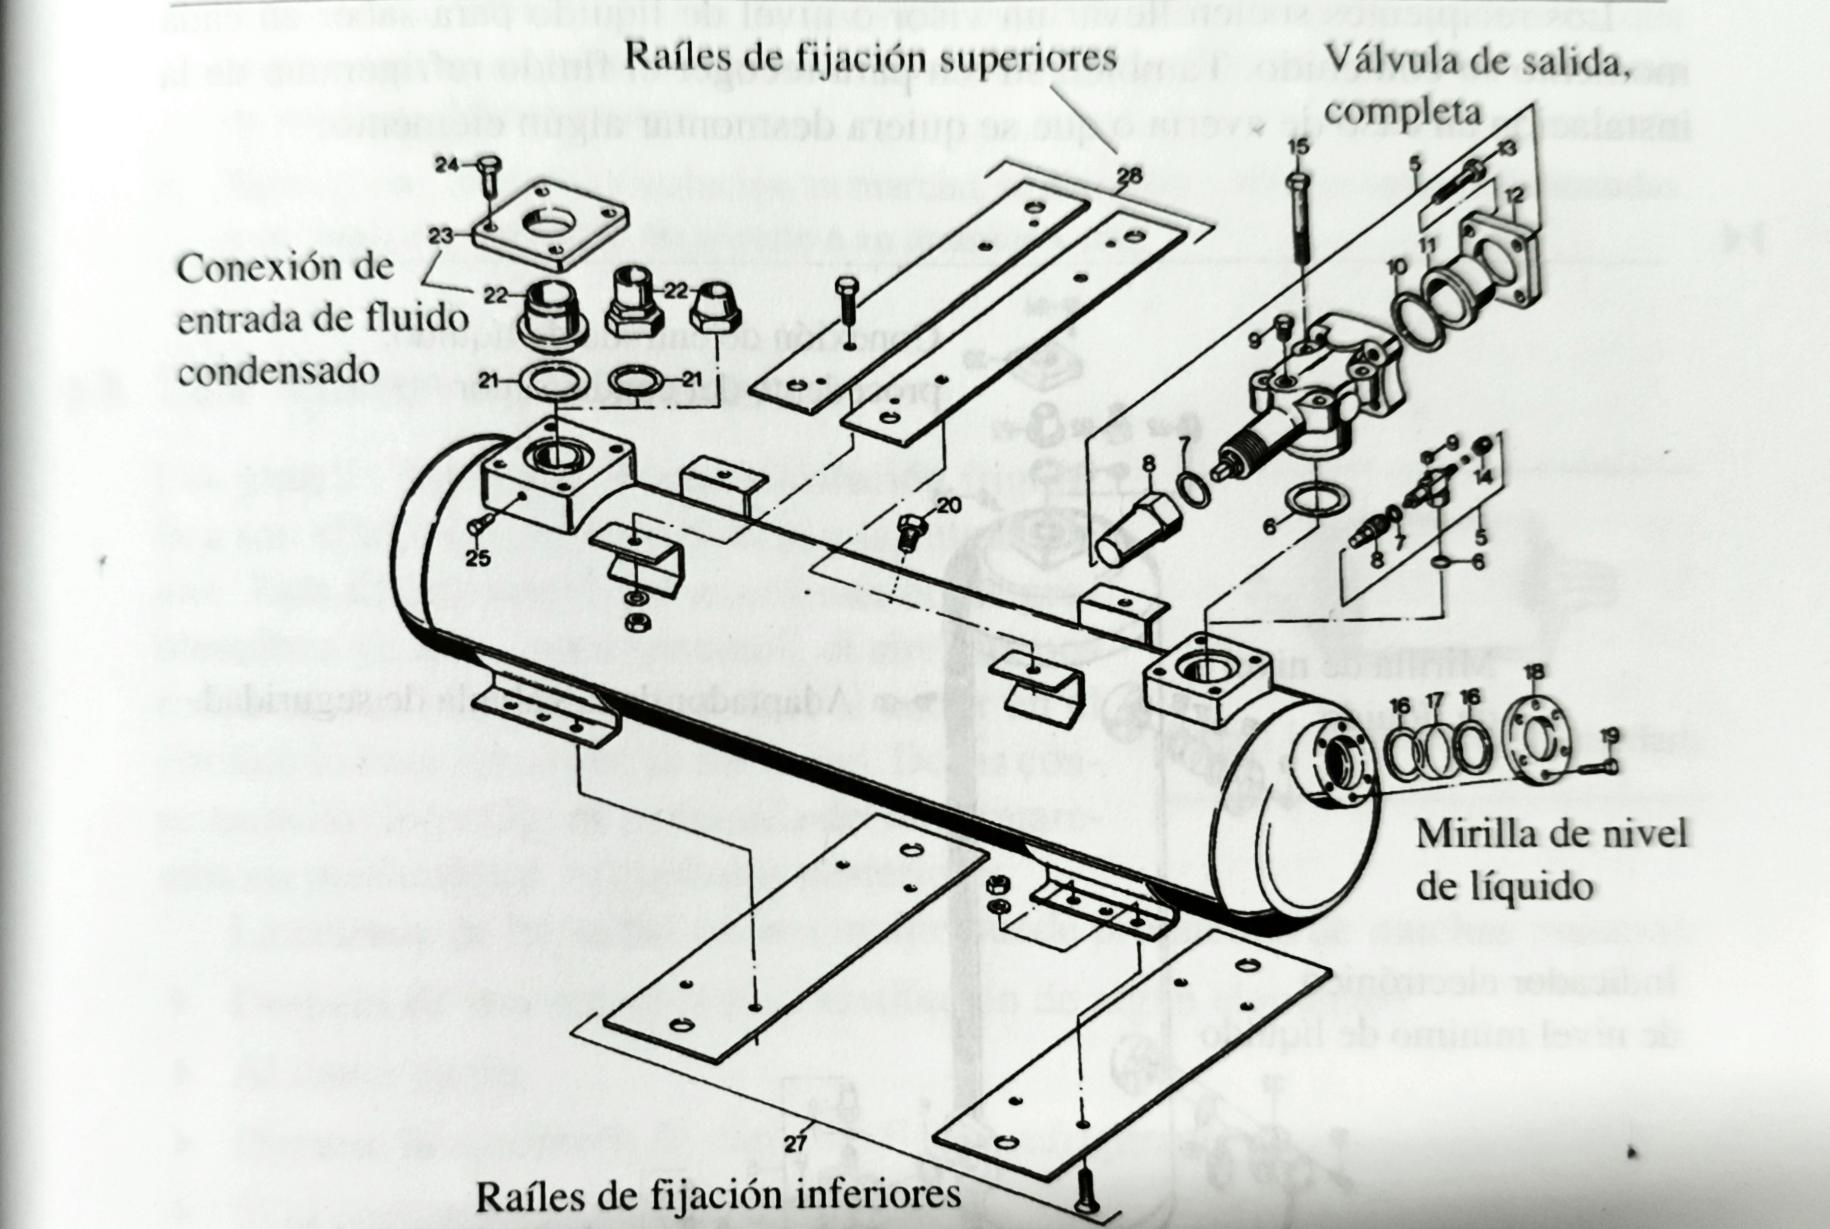
\includegraphics[width=0.7\textwidth]{figuras/recipiente horizontal.jpg}
	\caption{Recipiente de líquido horizontal}
	\label{fig:Recipiente de líquido horizontal}
\end{figure}

Al ser un recipiente de alta presión, debe llevar sus dispositivos de seguridad para evitar que se almacenen presiones peligrosas. También suelen llevar un visor o nivel de líquido para saber en cada momento su contenido.

\subsubsection{Filtros de humedad}

Los grandes enemigos de una instalación frigorífica son el temido golpe de líquido y la entrada de aire. Esta última implica a su vez la doble problemática, como sabemos, el aire que nos rodea es aire húmedo, con lo cual al entrar en el circuito lo hace junto con su humedad.

La entrada de humedad en un circuito puede producirse de muchas maneras:

\begin{itemize}
	\item Después de una reparación (o sustitución de un elemento)
	\item Al meter aceiteDurante la operación de carga de un fluido refrigerante
	\item Si el compresor aspira del aire ambiente
\end{itemize}

La humedad puede ocasionar serios problemas tales como bloquear los dispositivos de expansión (congelación de esas gotas del aire húmedo) o bien producir problemas en los compresores herméticos o semiherméticos, oxidaciones, etc. Para evitar la humedad en los circuitos se instalan unos filtros de humedad también llamados deshidratadores. Contienen un agente desecante que puede ser:

\begin{itemize}
	\item Silicagel
	\item Tamices moleculares
	\item Alúmina activada 
	\item Óxido de aluminio, muy empleado con los nuevos fluidos refrigerantes
\end{itemize}

También existen los denominados núcleo sólido, que son una mezcla de silicagel, tamices moleculares y óxido de aluminio.

Los filtros de humedad además de su función deshidratadora, retienen impurezas (partículas sólidas). 

A la hora de instalarse se deben seguir las intrucciones y el sentido de instalación indicado por el fabricante, si este sentido además es vertical desendente se aumentara el rendimiento del dispositivo.

\textit{La eficacia del agente desecante aumenta cuanto menor sea la temperatura del líquido a la entrada del filtro.} Supongamos, por ejemplo, una instalación con condensador por aire. En verano, al aumentar la temperatura ambiente, también aumenta la temperatura de condensación y por lo tanto la del líquido, lo que influye en la eficacia del agente deshidratador y puede provocar congelación en las válvulas de expansión. Por ello si se debiera instalar un intercambiador de calor, el filtro se montaría después.

\subsubsection{Visor}

De manera práctica diremos que es una ``ventana'' que tenemos en el circuito. A través de él deberíamos ver el fluido en estado líquido 100\% (saturado). Si, por ejemplo vemos burbujas, podría indicarnos que hace falta fluido refrigerante (poca carga, bien sea porque de origen no tiene la adecuada o por fugar posteriores) o bien, si hay burbujar y está frío, puede ser porque un estrangulamiento origina un expansión antes de llegar al visor. También nos indica si hay humedad en el circuit, ya que contiene una sal química higroscópica que reacciona con la humedad y cambia de color (no todos lo tienen).

\subsubsection{Acumulador de aspiración}

Es un elemento que se instala en el lado de baja presión, antes del compresor. Su función consiste en evitar que llegue el fluido en estado líquido al compresor. Es un recipiente metálico, que por lo general suele llevar un tubo de entrada y otro de salida. Evidentemente,\textit{el tubo de entrada se conecta a la tubería que viene del evaporador, y el de salida a la que va al compresor.}

No hay que confundir el acumulador de aspiración con el \textit{separador de líquido}, ya que éste es un elemento de las instaciones de régimen inundado y está perfectamente aislado, pues contiene el fluido expansionado a baja presión y temperatura.

\subsubsection{Intercambiador de calor}

Algunas instalaciones llevan intercambiadores de calor a contracorriente líquido-vapor de aspiración. Es decir, se produce intercambio de calor entre el líquido refrigerante procedente del recipiente y el vapor de salida del evaporador.

\begin{figure}[H]
	\centering
	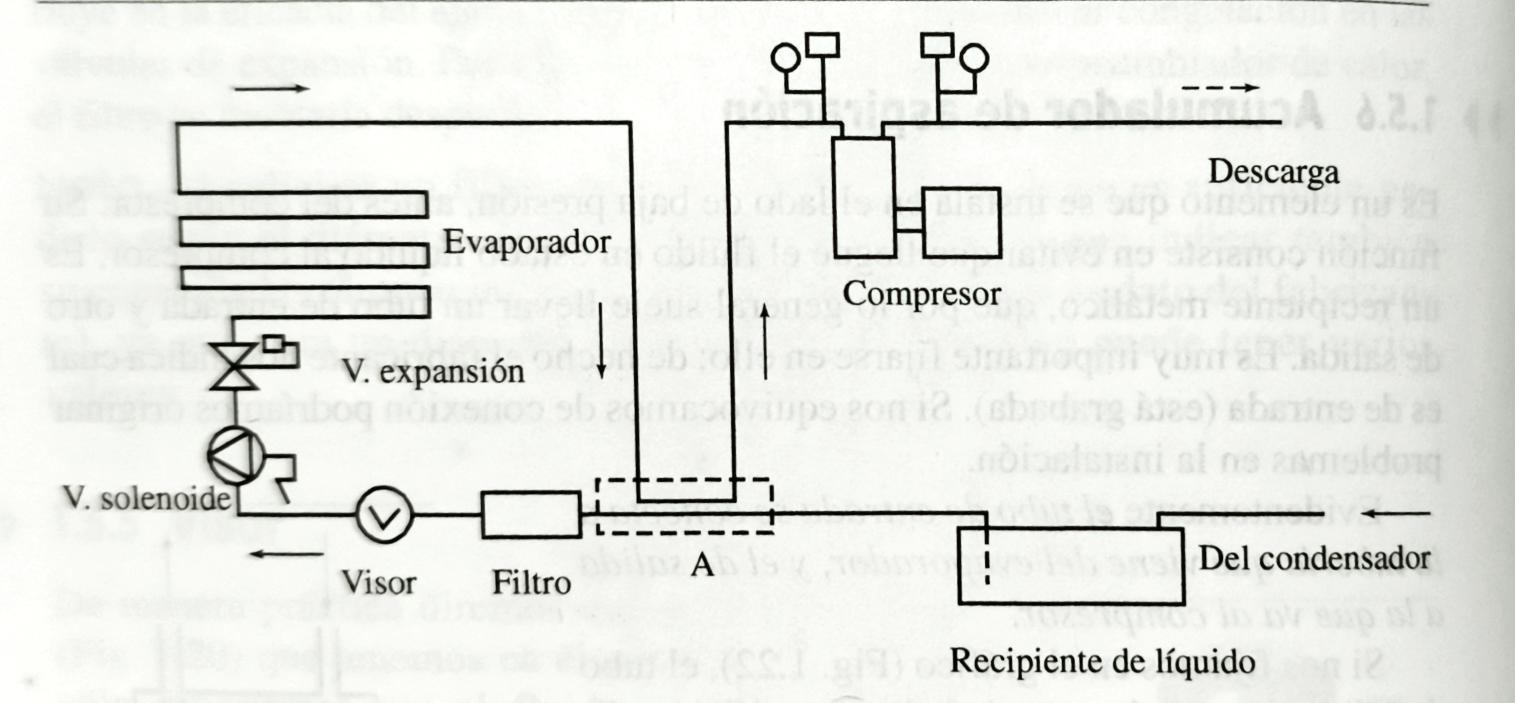
\includegraphics[width=\textwidth]{figuras/instalación con intercambiador.jpg}
	\caption{Instalación con intercambiador de calor}
	\label{fig:Instalación con intercambiador de calor}
\end{figure}

Al ser estos elementos intercambiadores de calor, tienen doble lectura:

\begin{enumerate}[a.]
	\item La del vapor frío de la aspiración que subenfría el líquido que va al dispositivo de expansión y aumenta el rendimiento dado que la temperatura con que entra el líquido en dicho dispositivo es menor (válvula de expansión en la \autoref{fig:Instalación con intercambiador de calor}).
	\item La temperatura del líquido que al estar en contacto con la tubería de salida del evaporador, vaporiza las posibles gotas de líquido que vayan al compresor, es decir evita que llegue líquido al compresor.
\end{enumerate}

 % Acá se habla del circuito básico y típico, los componentes que lleva y entre otras cosas
	
	\section{Diagramas de ciclos de refrigeración}\label{sec:1}

	En esta sección se utiliza como fuente principal el libro \emph{Principios de Refrigeración} de \cite[Capítulos 6 y 7]{dossat2004refrigeracion}.
	
	Los diagramas que con frecuencia se usan en el análisis del ciclo de refrigeración son los de \textit{presión-entalpia (ph)} y \textit{temperatura-entropía (Ts)}.
	
	%	Agregar gráfica de los diagramas ph y Ts para mostrar las regiones
	
	\subsection{Ciclo de refrigeración teórico} \label{sec:ciclo-teorico}
	
	%	Desarrollo del diagrama para un ciclo teórico
	
		El ciclo teórico es un ciclo de refrigeración saturado simple en el cual se supone que el vapor refrigerante que sale del evaporador y entra al compresor es vapor saturado a la temperatura y presión vaporizante, y el líquido refrigerante que sale del condensador y llega a la válvula de expansión es un líquido saturado a la temperatura y presión condensante. Además, se desprecian las pérdidas en las tuberías y en los accesorios.

		% Mencionar la disposición de los elementos y agregar la fig 7-5 del libro
		
		\begin{figure}[h]
			\centering
			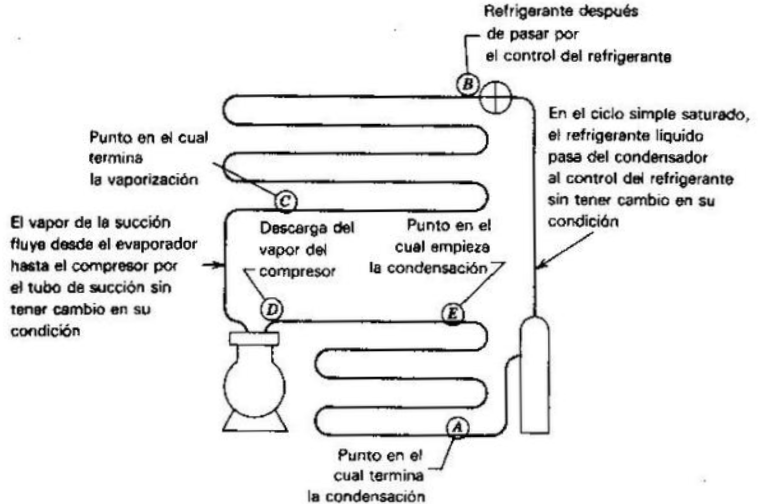
\includegraphics[width=.7\linewidth]{ciclo-saturado-simple}
			\caption{Diagrama de flujo de un ciclo saturado simple.}
			\label{fig:ciclo-teorico}
		\end{figure}
		
		\begin{figure}[h]
			\centering
			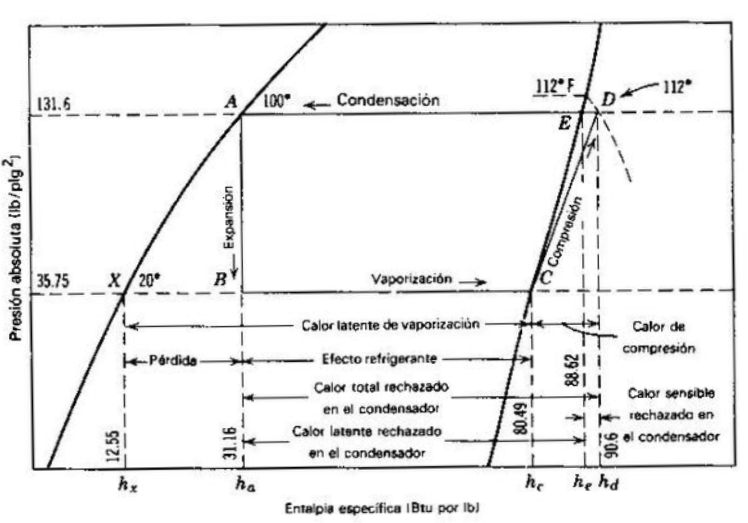
\includegraphics[width=.7\linewidth]{diagrama-ciclo-saturado-simple}
			\caption{Diagrama de flujo de un ciclo saturado simple.}
			\label{fig:diagrama-teorico}
		\end{figure}
		
		En el diagrama de la \autoref{fig:ciclo-teorico} se tiene el trazo de un ciclo saturado simple, y en la \autoref{fig:diagrama-teorico} se muestra un diagrama presión-entalpía de dicho ciclo, en el cual se observan cuatro transformaciones o procesos:
		
		\begin{itemize}
			\item Expansión.
			\item Evaporación.
			\item Compresión.
			\item Expansión.
		\end{itemize}
		
		\subsubsection{Proceso de expansión} El proceso de expansión es representado en el diagrama por el trazo $A-B$. Es un estrangulamiento tipo expansión adiabática y sucede en la válvula de expansión cuando la presión del líquido refrigerante es reducida desde la presión en el condensador a la presión en el evaporador. La temperatura del líquido que llega a la válvula de expansión A siempre es bastante mayor que la temperatura en el evaporador B y ésta deberá primero reducirse hasta dicha temperatura antes de que el líquido pueda vaporizarse en el evaporador.
			
			
			 
			En este ciclo teórico no hay ningún cambio en las propiedades del líquido refrigerante a medida que éste fluye a través de la línea de líquido desde el condensador a la válvula de expansión, y es la condición que se tiene en el punto A en el diagrama. 
			
				
				
			En este proceso, cuando el refrigerante que está a la temperatura y presión del punto A, pasa a través de la válvula de expansión, su presión se reduce a la presión del evaporador, y debe ceder suficiente calor para enfriarse a sí mismo desde la temperatura en A hasta la temperatura en B. Debido a que esta caída de presión ocurre instantáneamente, no se tiene tiempo para que tenga lugar una transferencia de calor entre el refrigerante y los alrededores. En consecuencia, el proceso es adiabático, y la disminución necesaria de temperatura del fluido se logra sólo por la transferencia de energía que se tiene dentro del fluido. Por esta razón, una parte de la masa líquida se cambia de inmediato a la fase de vapor, que se denomina \emph{vapor flash}. Esta parte que se vaporiza no produce enfriamiento útil y por lo mismo representa una pérdida de \emph{efecto refrigerante} en comparación con la suposición de que toda la masa fuera vaporizada en el evaporador.
			
			
			\subsubsection{Proceso vaporizante} El proceso $B-C$ se efectúa a presión y temperatura constantes y es la vaporización del refrigerante en el evaporador. 
			
			A medida que el refrigerante fluye a través del evaporador, este absorbe el calor del medio a refrigerar e incrementa su entalpía hasta el punto C donde estará completamente vaporizado, y es un vapor saturado a la temperatura y presión del evaporador.
			
			La distancia entre los puntos X y C en el diagrama \textit{ph} representa el calor latente total de vaporización. Entonces, ya que la distancia $B-C$ representa el efecto refrigerante, la distancia $X-B$ es la pérdida de efecto refrigerante.
				    
			\subsubsection{Proceso de compresión} En el ciclo teórico, se supone que el refrigerante mantiene sus propiedades a medida que atraviesa la línea de succión. El proceso $C-D$ se efectúa en el compresor a medida que el refrigerante incrementa su presión desde la presión del evaporador a la del condensador.
			
			En este proceso, no hay cambio en la entropía del refrigerante, por lo que, al alcanzar la presión del condensador, se encuentra en estado de vapor sobrecalentado.
				  
			\subsubsection{Proceso de condensación} El proceso $D-E$ toma lugar en una parte de la línea de descarga y en la parte superior del condensador. Esto representa el enfriamiento del vapor sobrecalentado hasta la temperatura condensante. Durante este proceso, la presión se mantiene constante. En el punto E, el refrigerante es un vapor saturado a la temperatura y presión condensante, o del condensador.
			
			El proceso $E-A$ es la condensación del vapor en el condensador y representa el calor cedido al medio exterior. 
			
			Al llegar al punto A, el refrigerante se encuentra como líquido saturado y ha completado un ciclo. Entonces, el calor total cedido por el refrigerante debe ser exactamente igual al calor absorbido en todos los demás puntos del ciclo. Por lo tanto,
			
			\begin{equation*}
				q_c = q_e + q_w
			\end{equation*}
			
			donde
			\begin{itemize}
				\item $q_c$ es el calor eliminado en el condensador,
				\item $q_e$ es el calor absorbido en el evaporador,
				\item $q_w$ es el calor absorbido equivalente debido al trabajo mecánico del compresor.
			\end{itemize}
			
	
	\subsection{Efecto de la temperatura en la eficiencia del ciclo}
	
		La eficiencia del ciclo de refrigeración compresión-vapor varía considerablemente tanto con la temperatura vaporizante como con la condensante\footnote{También se podría hacer referencia a la presión, debido a que para valores por debajo de la curva de saturación, la presión y temperatura se encuentran sobre la misma recta y permanecen constantes.}, siendo la temperatura del evaporador la que produce mayor efecto.
		
		\subsubsection{Efecto de la temperatura de succión}
		
		Si la temperatura condensante se mantiene constante, la eficiencia del ciclo disminuye al reducirse la temperatura vaporizante o de succión.\\
		
		
		Para mostrar el efecto que la temperatura de succión tiene sobre la eficiencia del ciclo, en la \autoref{fig:efecto-t-evaporador} se tienen los diagramas \emph{ph} de dos ciclos saturados simples trabajando a distintas temperaturas.
		
		\begin{figure}[h]
			\centering
			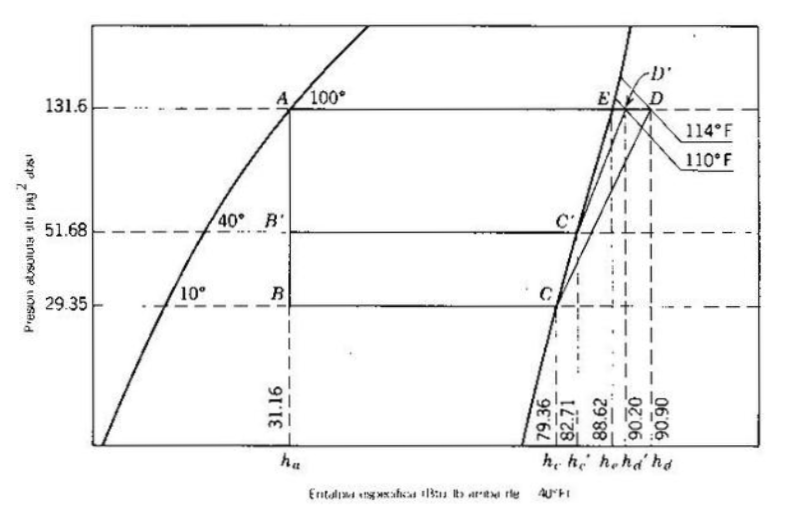
\includegraphics[width=.95\linewidth]{efecto-t-evaporador}
			\caption{Comparación entre dos ciclos saturados simples que trabajan a diferentes temperaturas vaporizantes.}
			\label{fig:efecto-t-evaporador}
		\end{figure}
		
		Uno de los dos ciclos identificados por los puntos A, B, C, D y E, el evaporador está trabajando a una temperatura de $10$ °F y el condensador a una temperatura de $100$ °F, y en los puntos A, B', C', D', y E, se tiene un ciclo similar que tiene la misma temperatura condensante pero que está trabajando a una temperatura vaporizante de $40$ °F.
		
%		Al comparar los dos ciclos se observa que el efecto refrigerante por unidad de masa es mayor para el ciclo que tiene mayor temperatura, esto debido a que se tiene un diferencial menor de temperatura entre la temperatura de baja y de alta.
		Al comparar los dos ciclos se observa que el efecto refrigerante por unidad de masa es mayor para el ciclo que tiene mayor temperatura de vaporización. Este hecho se debe a que el fluido debe ceder menos cantidad de calor para enfriarse a sí mismo a la temperatura del evaporador (proceso expuesto en la  \autoref{sec:ciclo-teorico}). \\
		
		
		\textit{En resumen, a mayor diferencial de temperatura o presión entre el condensador y el evaporador, menor será el efecto refrigerante por unidad de masa.}\\
		
		
		Por otro lado, el trabajo de compresión por unidad de masa necesario para comprimir al vapor desde la presión vaporizante hasta la presión condensante es menor para el ciclo de menor diferencial de temperatura.
		
		De manera similar, cuanto mayor sea el valor de caída de temperatura (o presión), mayor será el volumen específico y por tanto, menor será el desplazamiento volumétrico del compresor (la masa de refrigerante circulado por un compresor será menor)\footnote{En otras palabras, por cada kilogramo de refrigerante en circulación, el compresor deberá comprimir un volumen mayor de vapor.}.
		
		
		Cabe destacar que el aumento en porcentaje del volumen comprimido es mucho mayor que el aumento en porcentaje del caudal másico, lo cual, es probable que esto sea uno de los factores más importantes que influyen en la capacidad y eficiencia de un sistema de refrigeración y por consiguiente sea el más observado. Siguiendo el ejemplo expuesto en el libro (\cite[páginas 137 a 140]{dossat2004refrigeracion}), se observa que el aumento en masa es del $6.5\%$, mientras que el aumento en volumen es de $45\%$.
		
	
		\subsubsection{Efecto de la temperatura de descarga}
		
		En general, si la temperatura vaporizante se mantiene constante, disminuirá la eficiencia del ciclo al aumentarse la temperatura condensante.
		
		
		Para mostrar el efecto de la temperatura condensante sobre la eficiencia del ciclo, en la \autoref{fig:efecto-t-condensador} se muestra un diagrama \emph{ph} de dos ciclos diferentes. El ciclo A, B, C, D y E, es el cual tiene una temperatura condensante de $100$ °F, mientras que el ciclo A', B', C, D' y E', trabaja a $120$ °F.
		
		\begin{figure}[H]
			\centering
			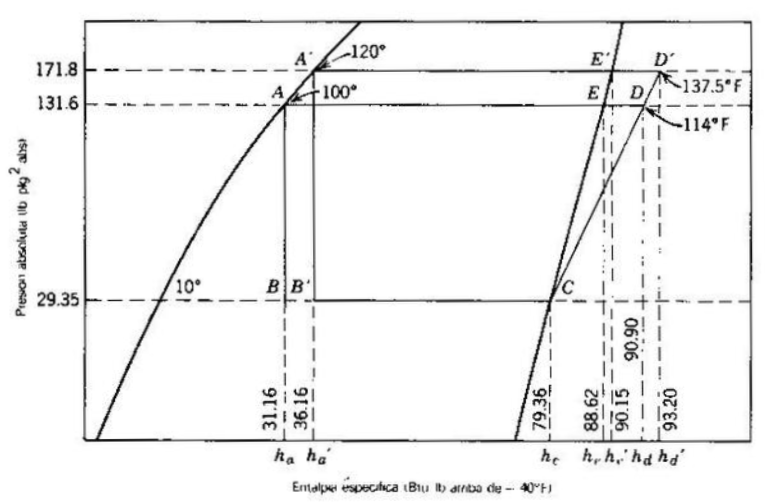
\includegraphics[width=.9\linewidth]{efecto-t-condensador}
			\caption{Comparación entre dos ciclos saturados simples que trabajan a diferentes temperaturas condensantes.}
			\label{fig:efecto-t-condensador}
		\end{figure}
		
		A medida que se aumenta la temperatura condensante, se aumenta también la temperatura que llega a la válvula de expansión y se reduce el valor del efecto refrigerante. En consecuencia, el caudal de masa del refrigerante será mayor.
		
		
		Ya que el caudal de masa es mayor para la temperatura condensante más alta, se deduce que el volumen de vapor comprimido es también mayor. Realizando un análisis, se puede observar que el aumento en porcentaje en el volumen de vapor manejado por el compresor es exactamente igual al porcentaje de aumento del caudal másico. Esto contrasta con lo que sucede cuando es variada la temperatura vaporizante.
		
		% 
		Por otro lado, debido a que la diferencia entre las presiones es grande, el trabajo de compresión por unidad de masa será mayor para el ciclo que tenga la mayor temperatura condensante. Como resultado de esto, la potencia teórica requerida también aumentará.
		
		
	\subsection{Ciclo de refrigeración real}
	
	Capítulo 9 del libro
	
		En los ciclos reales de refrigeración se tienen en cuenta ciertas consideraciones que no se contemplaron en el ciclo teórico, como la caída de presión que experimenta el fluido al paso por tuberías, evaporador, condensador, etc. Además, se considerará el subenfriamiento del líquido y el sobrecalentamiento del vapor en la tubería de succión.
		
		
		Los efectos que fueron despreciables en el ciclo teórico, y por tanto los que se considerarán en el ciclo real de refrigeración se enlistan a continuación:
		\begin{itemize}
			\item Sobrecalentamiento en el vapor de succión
			% 8-3 Sobrecalentamiento sin aprovechamiento del enfriamiento
			% 8-4 Sobrecalentamiento con aprovechamiento del enfriamiento
			% 8-5 Sobrecalentamiento en la tubería de succión (sí o sí es no aprovechado, debe aislarse la tubería): explicación de la generación de escarcha
			% 8-6 Sobrecalentamiento del vapor en el espacio refrigerado. Acá menciona la "tubería secadora"
			\item Subenfriamiento en el líquido
			% 8-7 Subenfriamiento en el líquido. Con subenfriador, o torre de enfriamiento
			% 8-8 Intercambiadores de calor. Se utilizan para subenfriar el líquido antes de la válvula de expansión. Ya que es inevitable el sobrecalentamiento del vapor de la succión en un ciclo real, sea que se uso o no un intercambiador de calor, vale la pena cualquier medio práctico que se emplee para aprovechar el enfriamiento del líquido que se tiene en el sobrecalentamiento del vapor.
			\item Pérdidas de fricción
			% 8-9 Pérdidas debidas a la fricción, en tuberías y en válvulas. Para cualquiera caso, en el lado de descarga del compresor la pérdida resulta en un aumento (inevitable) de presión y en el lado de succión, una disminución. En el resto de elementos siempre es una caída de presión. Ver diagrama
			
			
		\end{itemize}
	
	
	\section{Compresores}

Es el coraz\'on de la instalaci\'on. Su funci\'on, dentro del sistema de refrigeración, consiste en aspirar el fluido refrigerante a baja presi\'on y temperatura tales que se pueda condensar.

Lo escrito en esta secci\'on esta basado en el libro \textit{Manual de refrigeración} de \cite[cap\'itulo 3]{Franco2016Manual}.

Los tipos de compresores m\'as empleados en la refrigeración son:

\begin{itemize}
	\item Alternativos 
	\item De tornillo o helicoidales
	\item Rotativos
	\item Centr\'ifugos
\end{itemize}

\subsection{Alternativos}

Pueden ser de simple efecto o de doble efecto, seg\'un realice la compresi\'on del fluido en un solo lado del pist\'on o en ambos lados. Los m\'as utilizados son los de simple efecto.

\subsubsection{Elementos del compresor}

\textbf{Bloque}

El bloque aglutina y soporta todos los elementos del compresor, tanto como fijos como m\'oviles. La parte superior es la culata y la inferior, por su interior, el c\'arter.

\begin{figure}[H]
	\centering
	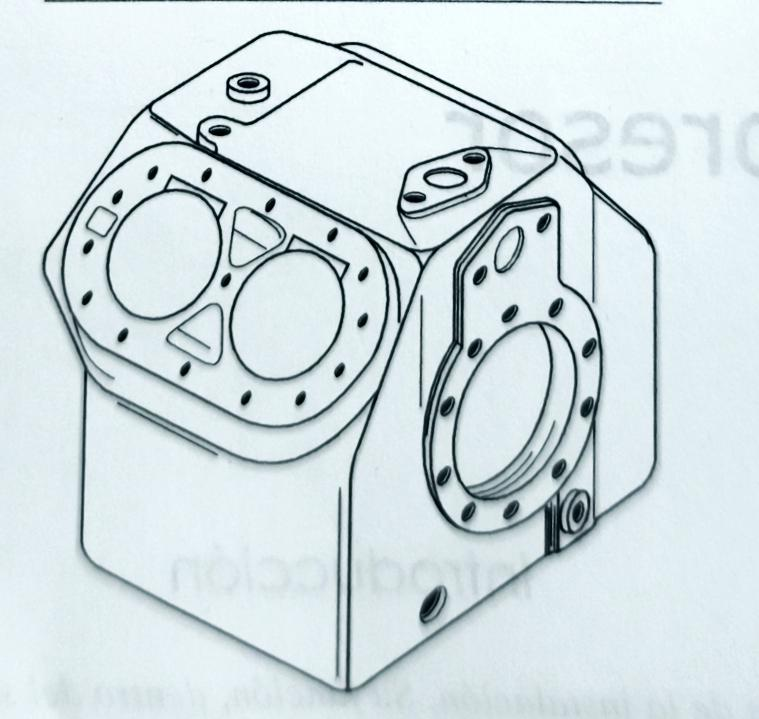
\includegraphics[width=.5\linewidth]{figuras/compresores/bloque}
	\caption{Bloque de un compresor}
	\label{fig:Bloque de un compresor}
\end{figure}

\textbf{C\'arter}

Es el espacio interior comprendido entre el eje cig\"ue\~{n}al y el fondo del bloque, destinado a almacenar el aceite de lubricación.

\textbf{Cilindro}
\begin{wrapfigure}{r}{0.4\linewidth}
	\centering
	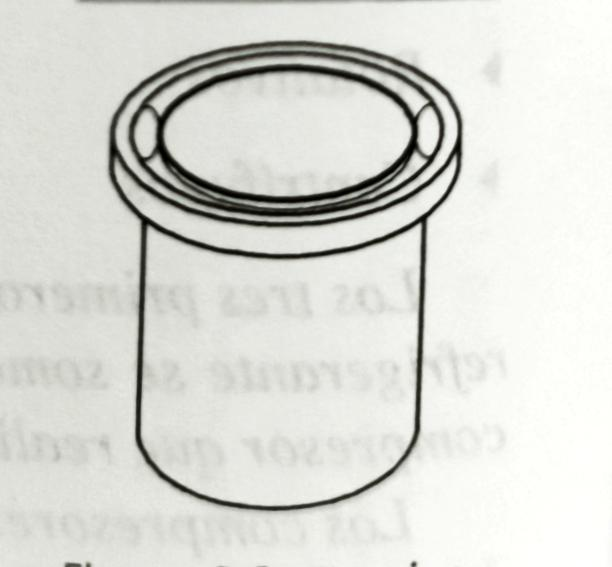
\includegraphics[width=.5\linewidth]{figuras/compresores/cilindro con camisa.jpg}
	\caption{Camisa}
	\label{fig:Camisa}
\end{wrapfigure}
Espacio donde va alojado el pist\'on. En su interior, \'este se desplaza en movimiento rect\'ilineo alternativo. En compresores de mediana y gran potencia (\autoref{fig:Camisa}) lleva camisa, que es una pieza cil\'indrica de acero que lo reviste, y que en casos de desgaste se puede rectificar, o sustituir si procede.

\textbf{Pist\'on o \'embolo}

Elemento que,desplaz\'andose en el interior del cilindro, provoca la aspiraci\'on, compresión y descarga del fluido refrigerante. Lleva alojados los aros o segmentos, que pueden ser:
\begin{itemize}
	\item Aros de engrase: Permiten la lubricación de los cilindros y, en su movimiento, arrastran el aceite al c\'arter.
	\item Aros de compresi\'on: Impiden que el fluido refrigerante escape por los espacios entre el pist\'on y el cilindro, hacia la parte inferior (c\'arter). Esto se aprecia mejor durante la compresi\'on, ya que si hay fugas no se alcanzan las altas presiones necesarias.
\end{itemize}
\textbf{Biela}\\
La biela (\autoref{fig:Conjunto biela-pist\'on y aros}) es el elemento que uno el pist\'on con el eje cig\"ue\~{n}al. Transforma el movimiento circular del eje cig\"ue~{n}al en rectil\'ineo alternativo del pist\'on. Por ello son resistentes y ligeras. La parte superior se llama pie de biela y se une al pist\'on por medio de un bul\'on para evitar el desplazamiento lateral de \'este. Y la parte inferior se llama cabeza de biela y se uno al eje cig\"ue\~{n}al. La biela puede ser de dos tipos, seg\'un se conecte al eje cig\"u\~{n}alo a una exc\'entrica.
\begin{figure}[H]
	\centering
	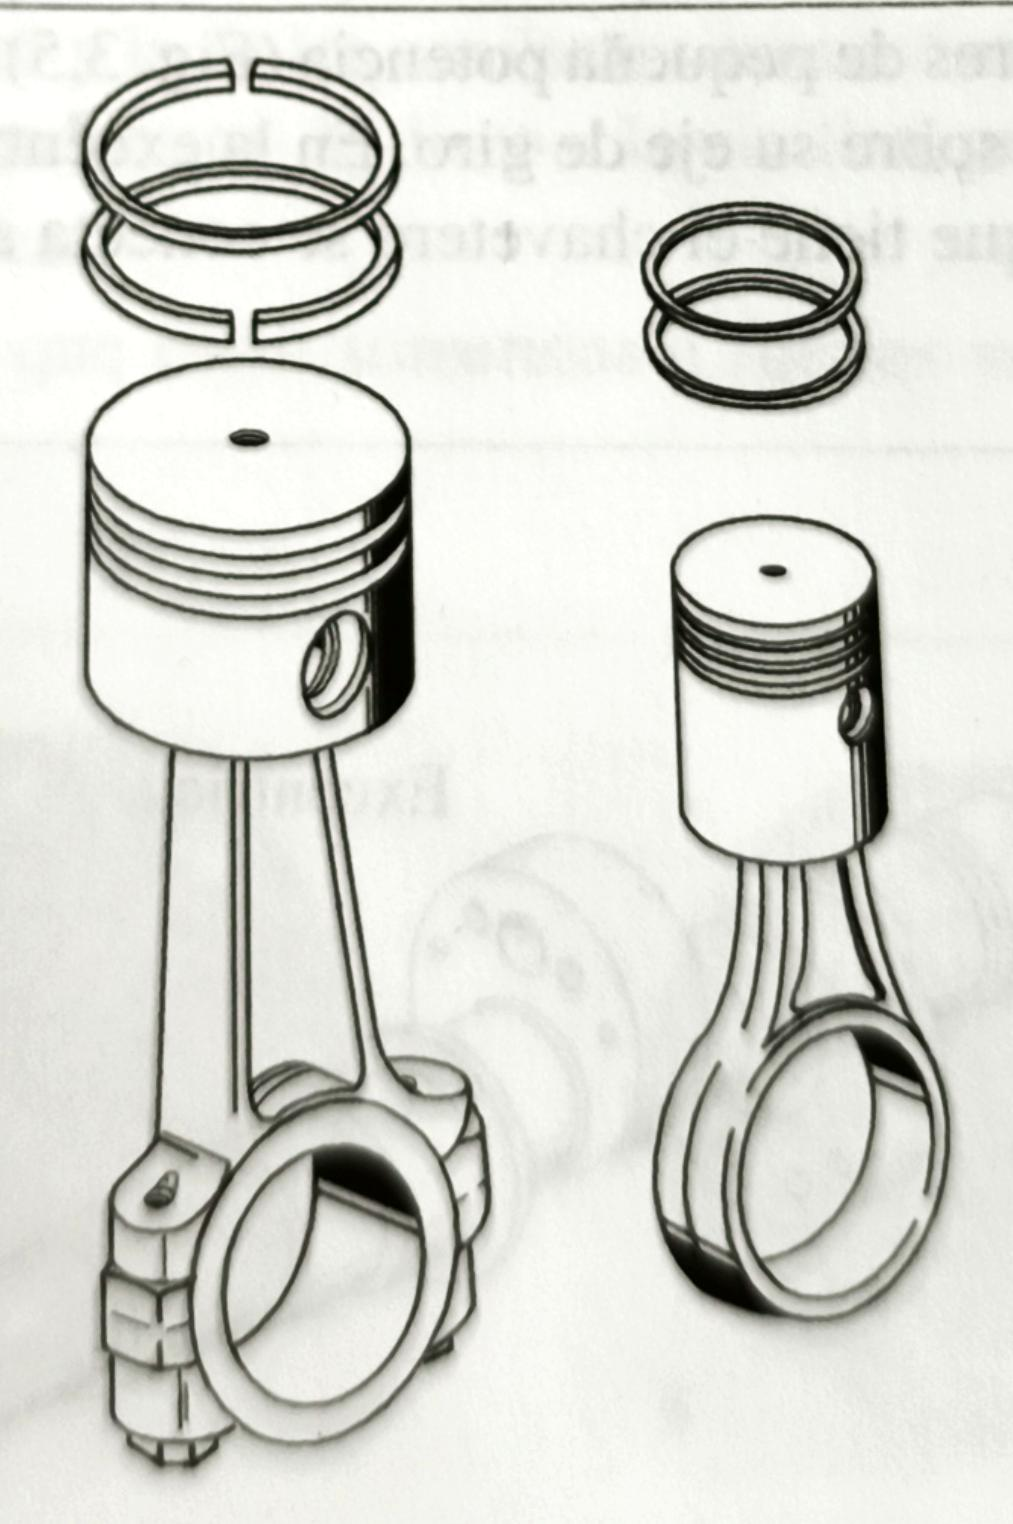
\includegraphics[width=.3\textwidth]{figuras/compresores/piston y biela.jpg}
	\caption{Conjunto biela-pist\'on y aros}
	\label{fig:Conjunto biela-pist\'on y aros}
\end{figure}

\textbf{Eje cig\"ue\~{n}al}\\
La disposici\'on y forma dependen del n\'umero de cilindros (\autoref{fig:Eje cigueñal}). Est\'a formado por un n\'umero determinado de manivelas, que tienen en sus respectivos lados opuestos unos contrapesos de equilibrado. La manivela es la part eque se coencta a la biela.\\
Los extremos del eje, llamados cuellos o mu\~{n}equillas, son los soportes que se apoyan sobe la bancada del compresor. El extremo del eje que tiene el chavetero es el que se conecta al motor el\'ectrico para su accionamiento. El otro extremo acciona la bomba de lubricación.
\begin{figure}[H]
	\centering
	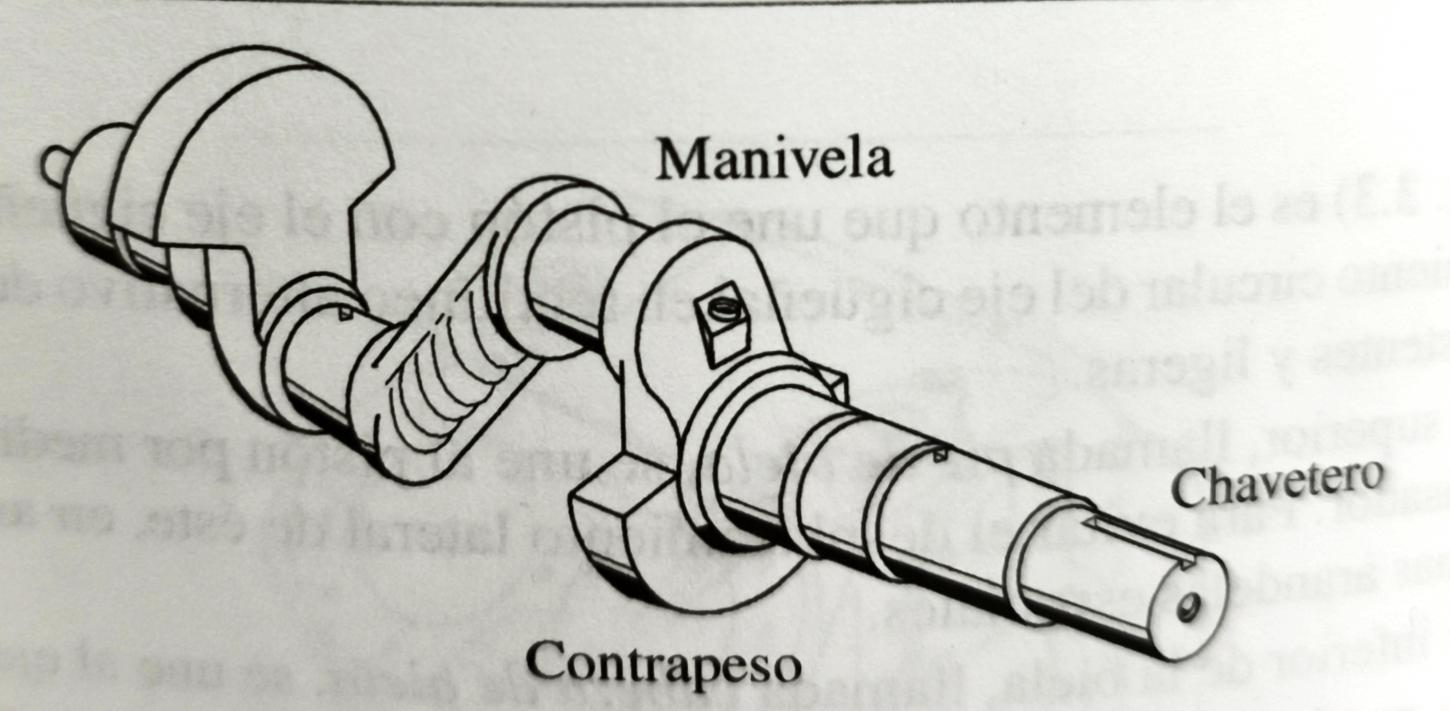
\includegraphics[width=.5\textwidth]{figuras/compresores/eje cigueñal.jpg}
	\caption{Eje cigueñal}
	\label{fig:Eje cigueñal}
\end{figure}
\textbf{Eje de exc\'entrica}\\
Se emplea en compresores de peque\~{n}a potencia (\autoref{fig:Eje de exc\'entrica}). Act\'ua de forma exc\'entrica, de ah\'i el nombre, sobre su eje de giro. En la exc\'entrica se monta la biela. El extremo del eje que tiene el chavetero se conecta al motor el\'ectrico.
\begin{figure}[H]
	\centering
	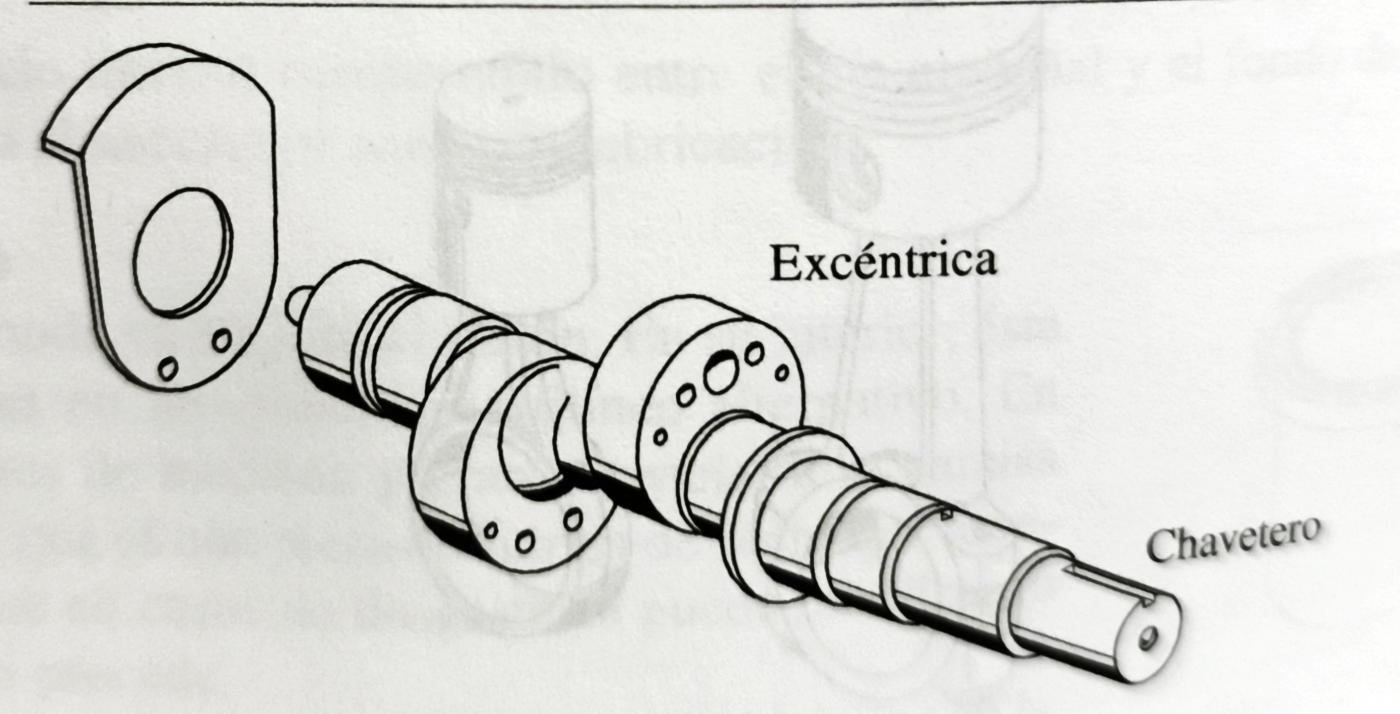
\includegraphics[width=.5\textwidth]{figuras/compresores/eje excentrico.jpg}
	\caption{Eje de exc\'entrica}
	\label{fig:Eje de exc\'entrica}
\end{figure}
\textbf{Culata}\\
Cierra el cilindro por la parte superior. Es la ``tapa'' del cilindro. En ella se alojan las v\'alvulas de aspiración y descarga. Como est\'a sometida a altas temperaturas puede ser refrigerada por aire o por agua (\autoref{fig:Culatas refrigeradas por aire y por agua}).
\begin{figure}[H]
	\centering
	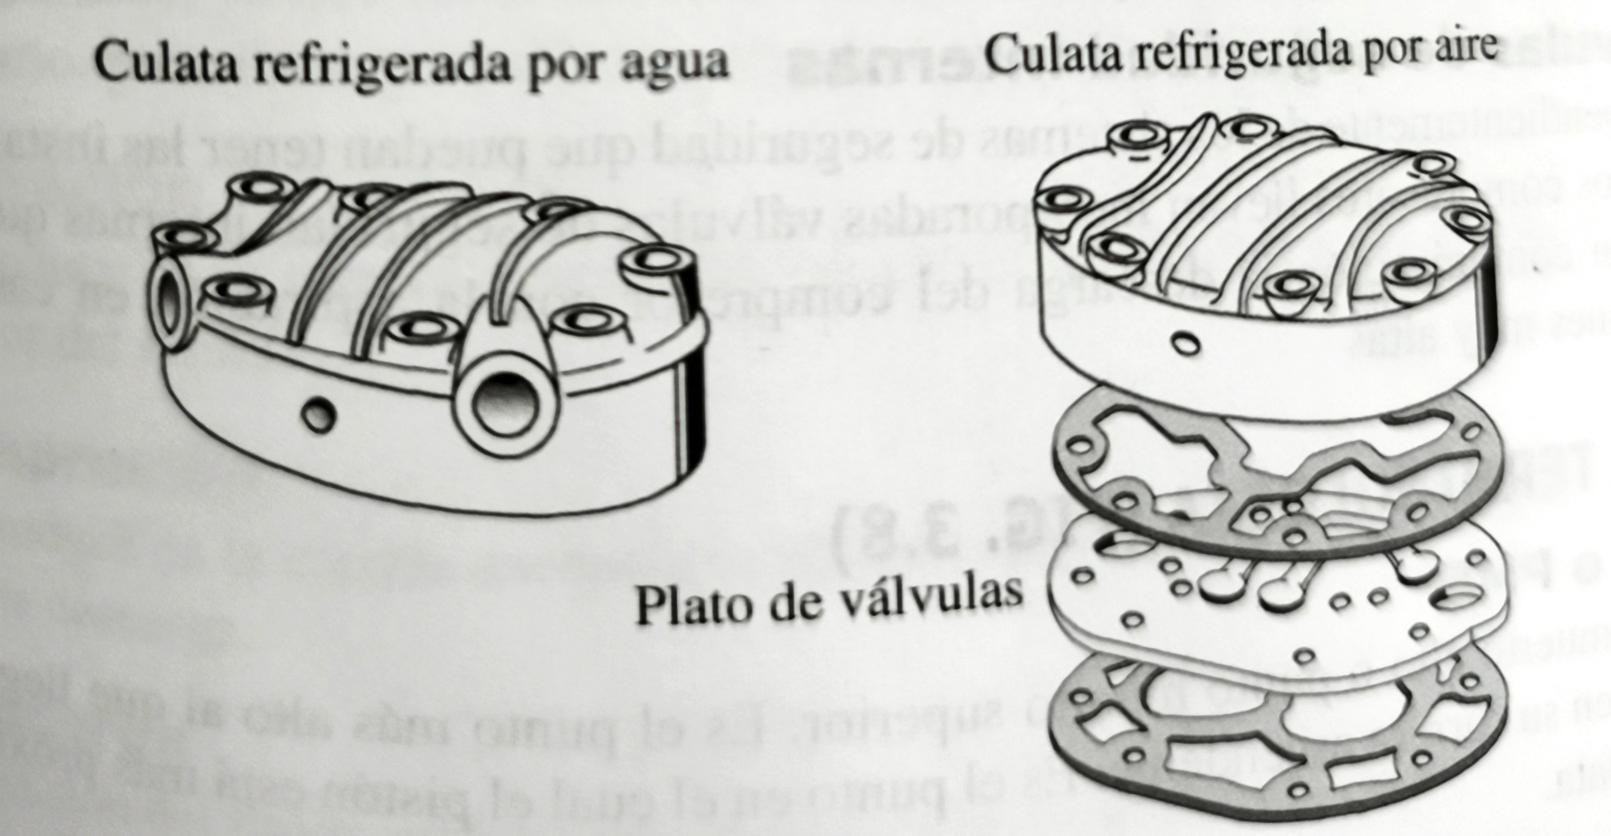
\includegraphics[width=.5\textwidth]{figuras/compresores/culata.jpg}
	\caption{Culatas refrigeradas por aire y por agua}
	\label{fig:Culatas refrigeradas por aire y por agua}
\end{figure}
\textbf{V\'alculas de aspiración y descarga}\\
Se encargan de comunicar el interior del cilindro con los conductos de aspiraci\'on y descarga. Su apertura y cierre se producen por la diferencia de presiones entre la del interior del cilindro y la de los conductos respectivos del fluido. Por lo general son de acero inoxidable, y para grandes potencias, dispotnen de resortes para su accionamiento.\\
\textbf{V\'alvulas de seguridad internas}\\
Independientemente de los sistemas de seguridad que puedan tener las instalaciones, los compresores llevan incorporadas v\'alvulas de seguridad internas que ponen en comunicaci\'on la descargas del compresor con la aspiración en caso de presiones muy altas.

%\subsubsection{Terminología}

%\textbf{PMA o PMS}\\
%Punto muerto alto o punto muerto superio. Es el punto m\'as alto al que llega el pist\'on en su carrera ascendente. Es el punto en el que \'el pist\'on est\'a m\'as cerca de la culata.\\
%\textbf{PMB o PMI}\\
%Punto muerto bajo o punto muerto inferior, es el punto m\'as bajo al que llega el pist\'on en su carrera.\\
%\textbf{Carrera}\\
%Distancia entre el PMS y el PMI. Corresponde a un \'angulo de giro de 180° del cig\"ue\~{n}al.
%
%\begin{figure}[H]
%	\centering
%	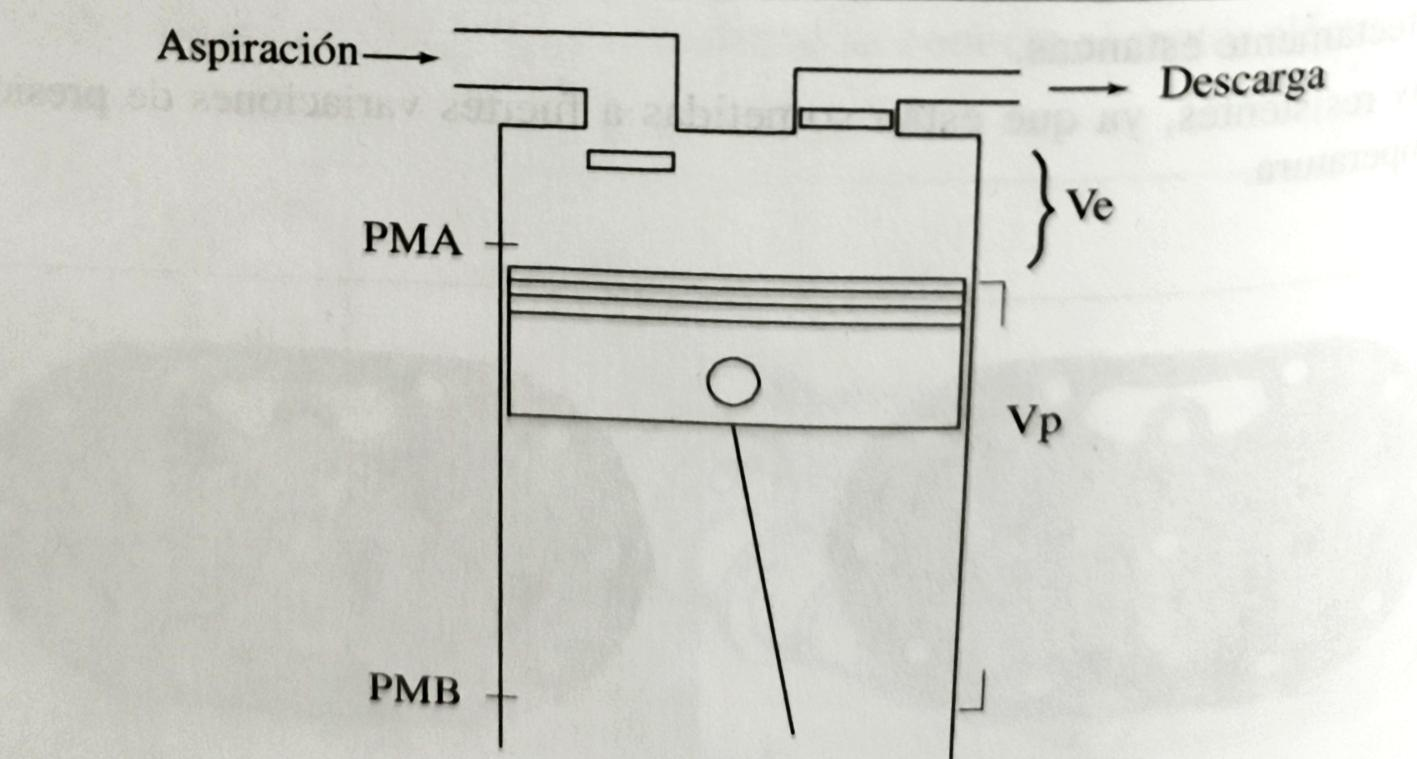
\includegraphics[width=.5\textwidth]{figuras/compresores/terminologia.jpg}
%	\caption{Terminolog\'ia de un cilindro en un compresor}
%	\label{fig:Terminolog\'ia}
%\end{figure}
%
%\textbf{Espacio neutro (Ve)}\\
%Es el comprendido entre el pist\'on cuando se encuentra en el PMS y la culata. Tambi\'en conocido como ``espacio muerto''.Tiene gran importancia en el rendimiento del compresor y est\'a determinado para evitar que el pist\'on, en su carrera ascendente, llegue a chocar con la culata, incluyendo las dilataciones que sufren los materiales, ya que est\'an sometidos a altas temperaturas. Debe ser el m\'inimo necesario, pues tiene gran repercusi\'on en el rendimiento volum\'etrico.\\
%\textbf{Aspiraci\'on}\\
%Se produce en la carrera descendente del pist\'on. Es la admisi\'on del fluido en el interior del cilindro.\\
%\textbf{Compresi\'on}\\
%Se produce en la carrera ascendente del pist\'on e inmediatamente despu\'es se realiza la descarga.\\
%\textbf{Descarga}\\
%Impulsi\'on del fluido refrigerante al conducto de descarga.\\
%\textbf{Volumen desplazado por el pist\'on (Vd)}\\
%El comprendido entre el PMS y PMI que desplaza el pist\'on en la carrera.\\
%\textbf{Volumen total del cilindro (Vt)}\\
%El comprendido entre el pist\'on cuando se encuentra en el PMI y la culata.
%\begin{equation*}
%	Vt = Ve + Vd
%\end{equation*}
%\textbf{Potencia indicada}\\
%Es la potencia que se genera en el interior del cilindro.\\
%\textbf{Potencia efectiva}\\
%Es la potencia que se debe suministrar con el motor el\'ectrico para que el compresor trabaje en las condiciones previstas. Es decir, es la potencia medida en el eje del compresor. Pero a partir de este punto se produce una disminuci\'on de la potencia ya que una parte de la misma se pierde en vencer los rozamientos de cojinetes, bielas, etc. Por ello, la potencia efectiva siempre ser\'a superior a la potencia indicada.
%\begin{equation*}
%	Pe > Pi
%\end{equation*}
%La potencia efectiva es la potencia de accionamiento.\\
%\textbf{Rendimiento mec\'anico}\\
%Es el valor que contempla las p\'erdidas de origen mec\'anico anteriormente mencionadas. Por lo tanto, es la relaci\'on entre ambas potencias:
%\begin{equation*}
%	\eta m = \frac{Pi}{Pe}
%\end{equation*}
\subsubsection{Funcionamiento}
Para facilitar su comprensi\'on vamos a ver como se producen los movimientos de apertura y cierre de las v\'alvulas de aspiraci\'on y descarga, con relaci\'on al movimiento del pist\'on.
\begin{enumerate}[a.]
	\item Carrera descendente:\\ Cuando el pistçón inicia la carrera descendente, hacia el PMI, crea en el interior del cilindro una depresi\'on que implica, que en su interior la presi\'on sea inferior a la existente en la parte superior de la v\'alvula, es decir en el conducto de aspiraci\'on, con lo que la v\'alvula de aspiraci\'on se abre (``baja'') y el fluido refrigerante entra en el cilindro.\\ El fluido entrar\'a en el cilindro hasta que se igualen las dos presiones, y en teor\'ia deber\'ia ser en cantidad igual a la correspondiente al volumen del cilindro, pero hay factores que impiden que entre esa cantidad.\\ La v\'alvula de descarga permanece cerrada, por la alta presi\'on existente en el conducto de descarga mientras el pist\'on se va acercando al PMI y la v\'alvula de aspiraci\'on contin\'ua abierta.\\ As\'i, cuando el pist\'on llega al PMI, la v\'alvula de aspiraci\'on est\'a abierta y la de descarga cerrada. El cig\"ue\~{n}al ha girado 180°.
	\item Carrera ascendente:\\ Cuando el pist\'on rebasa el PMI se inicia la carrera ascendente, y la v\'alvula de aspiraci\'on se cierra, porque la presi\'on en el interior del cilindro es superior a la existente en el conductor de aspiraci\'on. Con las dos v\'alvulas cerradas se inicia la compresi\'on del fluido (\autoref{fig:Carrera ascendente}A), y se produce:
	\begin{itemize}
		\item Una disminici\'on de volumen.
		\item Un aumento de la presi\'on y la temperatura, hasta que la primera alcanza un valor tal que hace que se abra (levante) la v\'alvula de descarga.
	\end{itemize}
	En la \autoref{fig:Carrera ascendente} se puede apreciar que poco antes de que el pist\'on llegue al PMS la v\'alvula de descarga abre (``hacia afuera''), porque la presi\'on en el interior del cilindro, en la carrera escendente, es superior a la del conducto de descarga y ``levanta'' la v\'alvula. El fluido es impulsado hacia el condensador.\\
	El cig\"ue\~{n}al ha girado 180°, con lo que las dos carreras consecutivas gir\'o 360°, es decir una vuelta.\\ Una vez rebasado el PMS, y con la v\'alvula de descarga cerrada, se reinicia el ciclo.
\end{enumerate}
\begin{figure}[H]
	\centering
	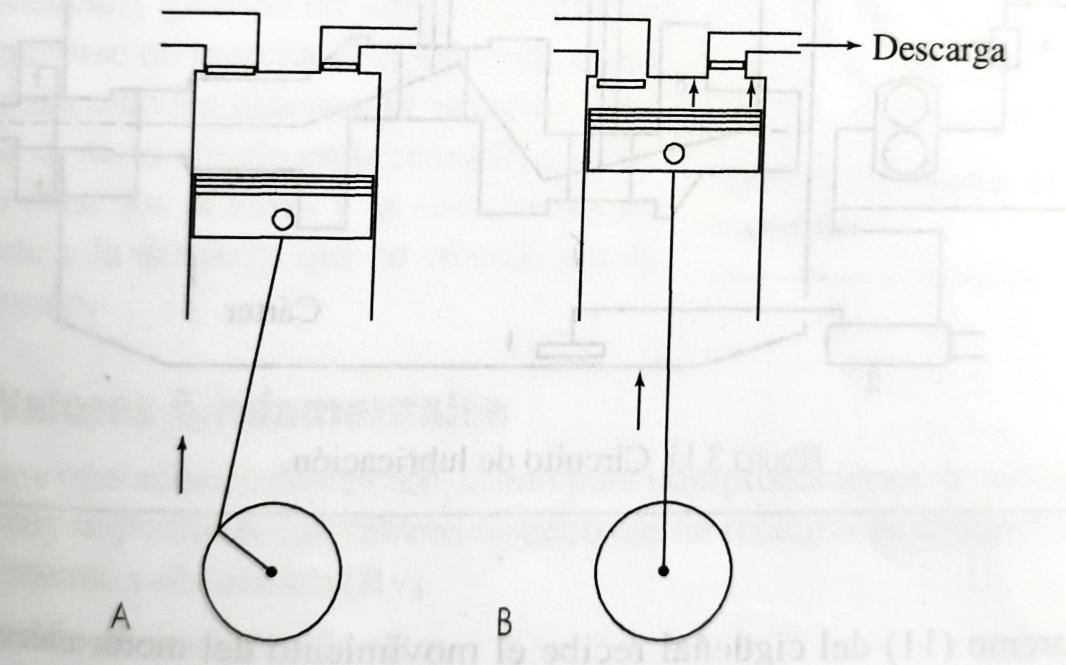
\includegraphics[width=.5\linewidth]{figuras/compresores/aspiracion y descarga.jpg}
	\caption{A = Compresi\'on. B = Descarga}
	\label{fig:Carrera ascendente}
\end{figure}
\subsubsection{Lubricación}
Es uno de los asprectos m\'as importantes del compresor y por lo tanto de la instalaci\'on. El tipo de lubricaci\'on empleada es forzada, mediante una bomba de engranajes que es accionada por el mismo motor el\'ectrico que acciona el compresor.\\ Anteriormente hemos comentado que a trav\'es de los aros de engrase, el aceite sale impulsado hacia las camisas. Pero tambi\'en se lubrican otras partes en movimiento como el cigueñal, cojinetes de bancada, cojinetes de biela y prensas principales.

Es importante saber que el circuito de aceite que conecta la bomba de engranajes con los dispositivos a lubricar cuenta con filtros y un enfriador de aceite, ya que este, adem\'as de lubricar, refrigera los elementos. El compresor tendr\'a enfriador de aceite dependiendo de su potencia, tipo y caracter\'isticas de funcionamiento.
\subsubsection{Valores fundamentales}
Tanto para operaciones de c\'alculo, como para comprobaciones de funcionamiento, son muy importantes los valores respectivos de relaci\'on de compresi\'on (Rc) y de rendimiento volum\'etrico (Rv).
\begin{enumerate}[1.]
	\item \textbf{Relaci\'on de compresi\'on (Rc)}
	\begin{equation*}
		Rc = \dfrac{\text{Presi\'on de descarga absoluta}}{\text{Presi\'on de aspiraci\'on absoluta}}
	\end{equation*}
	$\text{Presi\'on absoluta = Presi\'on manom\'etrica + Presi\'on atmosf\'erica}$
	\item \textbf{Rendimiento volum\'etrico (Rv)}\\ Se puede expresar de varias maneras, pero una de ellas a efectos pr\'acticos es:
	\begin{equation*}
		Rv = {\frac{\text{Volumen de vapor que realmente aspira}}{\text{Volumen te\'orico que tendr\'ia que aspirar}}X 100}
	\end{equation*}
	Cuanto mayor sea la relaci\'on de compresi\'on, menor ser\'a el rendimiento volum\'etrico y viceversa.

	Su valor depende de factores rales como el espacio neutro y la densidad del fluido en el interior del cilindro.
	\item \textbf{Volumen desplazado}\\ El volumen de fluido que en teor\'ia tiene que aspirar es el volumen desplazado por el pist\'on en su carrera. Como sabemos, el volumen de un cilindro es el producto del \'area por la altura:
	\begin{gather*}
		V = S \times h\\ 
		S = \pi\cdot r^2 = \pi\cdot(\frac{D}{2})^2 = \pi\cdot\frac{D^2}{4}
	\end{gather*}
	y la altura (h) es la distancia entre PMI y el PMS, o sea es la carrera:
	\begin{equation*}
		V = \frac{\pi D^2}{4}C
	\end{equation*}
	que es el volumen que desplaza el pist\'on en una revoluci\'on. Si gira el cig\"ue\~{n}al a n revoluciones por minuto y tiene N cilindros, el volumen desplazado ser\'a:
	\begin{equation*}
		Vd = \frac{\pi\cdot D^2\cdot C\cdot n\cdot N\cdot 60\cdot 10^-3}{4}(\frac{m^3}{h})
	\end{equation*}
\end{enumerate}
\subsection{Compresores herméticos}
Su \'ambito de aplicaci\'on comprende los sitemas de refrigeraci\'on y aire acondicionado.\\El motor el\'ectrico va acoplado directamente al compresor, y ambos dentro de la misma envolvente (carcasa) de acero formando una unidad. Al ser herm\'eticos (cerrados) no podemos acceder a ellos, como por ejemplo, para realizar operaciones de mantenimiento. Pueden ser alternativos, rotativos o de tornillo.\\ En su configuraci\'on (\autoref{fig:Compresor herm\'etico}), lleva tres tubos soldados a la carcasa. Dos son del mismo di\'ametro y el tercero menor. El de menor di\'ametro se conectar\'a a la descarga y la aspiraci\'on a cualquiera de los otros dos. Por lo general, se hace al tubo que est\'a al lado contrario de la placa de conexionado el\'ectrico, para evitr que las condensaciones que se puedan producir en el exterior del mismo, lleguen a introducirse a la placa.\\ De esta manera el otro tubo, que no se conecta la circuito, se puede utilizar para que, despu\'es de instalar una conexi\'on ob\'us o una v\'alvula de intervenci\'on, se aproveche para realizar operaciones tales como:
\begin{itemize}
	\item Meter carga de refrigerante
	\item Comprobar la presi\'on de aspiraci\'on
	\item Comprobar la temperatura de evaporaci\'on
	\item Meter aceite
\end{itemize}
\begin{figure}[H]
	\centering
	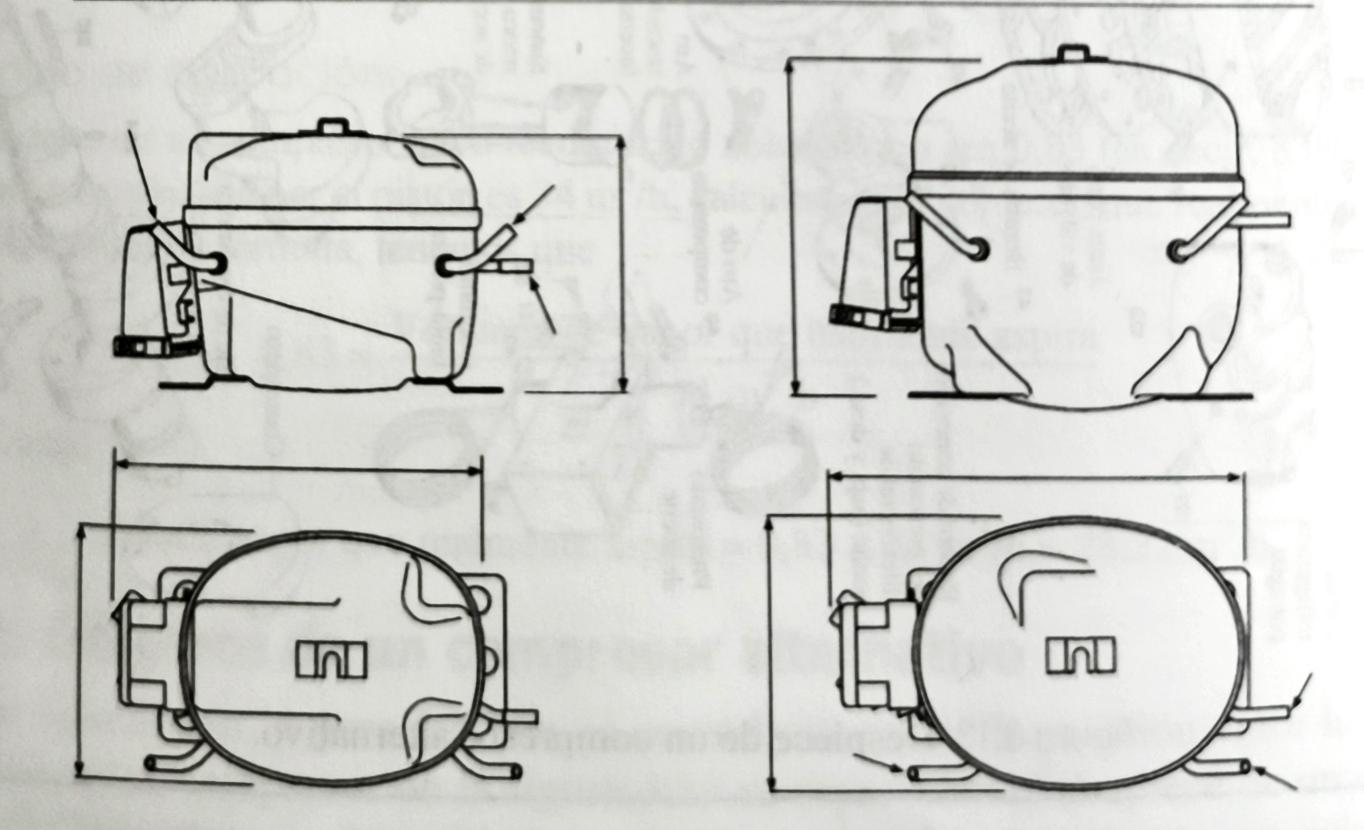
\includegraphics[width=.8\linewidth]{figuras/compresores/compresor herméticos.jpg}
	\caption{Compresor herm\'etico}
	\label{fig:Compresor herm\'etico}
\end{figure}
\subsubsection{Algunas caracter\'isticas}
\begin{enumerate}[1.]
	\item Son silenciosos porque cuentan con resortes interiores y c\'amaras silenciadoras que amortiguan el golpeteo de las v\'alvulas. Carecen de transmisiones exteriores como por ejemplo correas.
	\item Est\'an refrigeradores por el fluido de aspiraci\'on por lo que, la falta de fluido afectar\'ia a la refrigeraci\'on del compresor. Hay que evitar la humedad en el circuito y la entrada de l\'iquido al compresor porque estar\'ian en contacto con la parte el\'ectrica.
	\item Trabajar a temperaturas inferiores a las normales, implicar\'ia el aumento del volumen espec\'ifico, que afectar\'ia, entre otras cosas a la refrigeraci\'on.
\end{enumerate}
\subsection{Compresores semiherméticos}
Estos compresores en su funcionamiento tienen las mismas ventajas e inconvenientes que los herm\'eticos pero a diferencia que son m\'as accesibles para realizar mantenimiento. Por ejemplo, en compresores semiherm\'eticos alternativos se pueden desmontar para realizar operaciones de mantenimiento tales como cambiar pistones o aros.\\ Pueden ser enfriados externamente por aire o por agua.
\subsubsection{\'Acidos}
Es importante comentar que en los compresores, ya sean herm\'eticos o semiherm\'eticos, una de las aver\'ias m\'as importantes es la contaminaci\'on del circuito por \'acidos, puesto que se refrigeran por los vapores de aspiraci\'on. La presencia de \'acidos se produce por altas temperaturas en la zona que se encuentra entre el estator y rotor, esto genera que el fluido refrigerante reaccione y ataque los devanados del estator.\\ Las causas pueden ser varias pero se podr\'ia englobar en mantenimiento inadecuado, sobre carga del motor y elevadas temperaturas de trabajo.\\ Si se cambia un compresor por otro en un sistema contaminado por \'acidos y antes no se eliminan \'estos, atacar\'an a los aislamientos de los bobinados, con lo cual la duraci\'on del nuevo compresor ser\'a muy corta.
\subsection{Compresores abiertos}
Se llaman abiertos porque el motor el\'ectrico y el compresor est\'an separados. Por lo tanto, el fluido refrigerante ya no est\'a en contacto con la parte el\'ectrica, como ocurre en los compresores herm\'eticos y semiherm\'eticos. Como est\'an separados la conexi\'on entre ambos necesita de un sistema de estanqueidad o sello en ese punto para evitar las fugas del fluido refrigerante al exterior. El acoplamiento motor-compresor se puede realizar mediante correas, se puede adaptar la velocidad con sus di\'ametros (seg\'un necesidad de carga) o mediante dos platos met\'alicos unidos el\'asticamente.
\subsubsection{Caracter\'isticas de funcionamiento}
En estos compresores abiertos se considera buena relaci\'on de compresi\'on (Rc) si no excede de 10:1, ya que cuanto menor sea, mayor ser\'a el rendimiento volum\'etrico (Rv) y, por lo tanto, mayor ser\'a la potencia frogir\'ifica.\\ Si el compresor tuviera que trabajar con una Rc elevada, como sucede, por ejemplo, cuando se trata de instalaciones que necesiten temperaturas muy bajas para enfriar y las de condensaci\'on sean normales, entonces no se podr\'ia utilizar uno de simple etapa, porque entre otras cosas, las altas temperaturas afectar\'ian:
\begin{itemize}
	\item A los materiales (dilataciones)
	\item A la lubricaci\'on, perjudicar\'ia la viscosidad del aceite
	\item A las temperaturas de descarga, porque ser\'ian muy altas
	\item Y a los rendientos, que disminuir\'ian
\end{itemize}
Para solucionar estos inconvenientes tendr\'iamos que recurrir a los compresores de doble etapa (sistema compound), que tambi\'en se hace extensivo a los semiherm\'eticos.
\subsubsection{Compresores de doble etapa}
Los compresores de doble etapa reparten la elevada relaci\'on de presiones y disminuyen el alto recalentamiento. Cada secci\'on del compresor trabaja a menor presi\'on y tambi\'en menor temperatura de descarga, lo que implica un mejor aprovechamiento volum\'etrico. Para ello emplean un sistema de enfriamiento en la etapa intermedia, cuando es asi se los llama sistema por \textbf{inyecci\'on parcial}. Pero cuando se enfria el fluido en la etapa intermedia y, a su vez, antes de que \'este entre en el evaporador se lo llama sistema de \textbf{inyecci\'on total}.
\begin{itemize}
	\item \textbf{Inyecci\'on parcial:}\\ Se mezclan el fluido expansionado por la v\'alvula y los gases de descarga de los cilindros de baja en la tuber\'ia de presi\'on intermedia. De esta manera, se logra bajar la temperatura de descarga de los cilindros de alta.
	\item \textbf{Inyecci\'on total}\\ Se realiza un enfriamiento de los gases de descarga de los cilindros de baja y, a su vez, tambi\'en se hacen pasar el fluido expansionado por un intercambiador de calor para enfriar el refrigerante antes de entrar al evaporador e incrementar el efecto frigorífico.
\end{itemize} 
\subsection{Compresores rotativos}
Se caracterizan por comprimir el fluido refrigerante mediante el movimiento circular continuo de un rotor, que puede ser de exc\'entrica o de paletas.
\subsubsection{De exc\'entrica}
\begin{wrapfigure}{r}{0.45\linewidth}
	\centering
	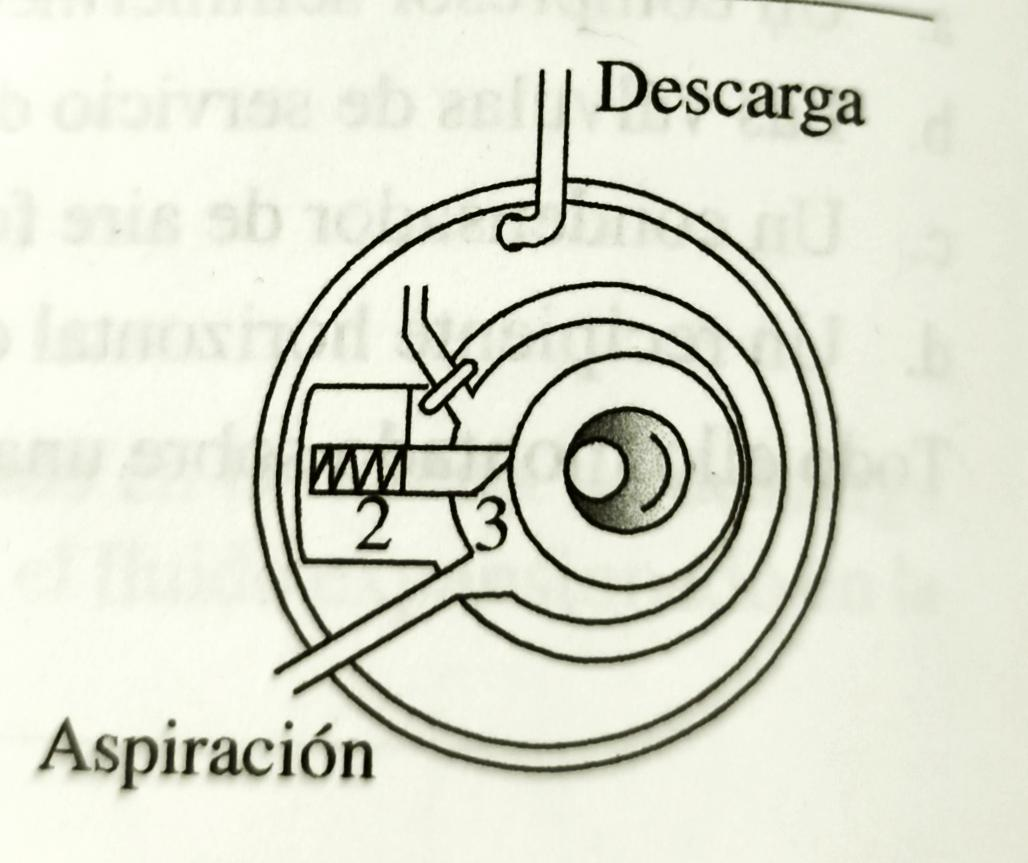
\includegraphics[width=.7\linewidth]{figuras/compresores/rotor de excentrica.jpg}
	\caption{Rotor de exc\'entrica}
	\label{fig:Rotor de exc\'entrica}
\end{wrapfigure}
Consta (\autoref{fig:Rotor de exc\'entrica}) de un rotor exc\'entrico respecto al cilindro donde se aloja y que en su movimiento llega a establecer contacto con \'el.\\Este rotor, por acci\'on del resorte (2) est\'a permanentemente en contacto con una paleta (3).\\Esta paleta, tal como se aprecia en la figura, establece la separaci\'on entre las c\'amaras de aspiraci\'on y de descarga. En su funcionamiento, la aspiraci\'on se realiza de manera continua, y al disminuir el espacio comprendido entre el rotor y el cilindro, se efect\'ua la comprensi\'on del fluido refrigerante y posterior descarga.

\subsubsection{De paletas}

B\'asicamente (\autoref{fig:Rotor de paletas}) consta de un rotor montado en el interior de un cilindro y cuyos centros ent\'an ligeramente desplazados. Este rotor aloja unas paletas que est\'an comprimidas contra la pared del cilindro por medio de unos resortes. Al pasar cada paleta por el orificio de la aspiraci\'on, se crea una depresi\'on que provoca la entrada del fluido en el espacio comprendido entre esa paleta y la anterior. Posteriormete y dado que el espacio entre el rotor y el cilindro disminuye, tambi\'en lo hace el volumen del fluido (compresi\'on) hasta que alcanza el orificio de descarga.\\ Existen compresores cuyos rotores no llevan resortes y las paletas se mantienen comprimidas por la acci\'on de su propio peso y de la fuerza centr\'ifuga.

\begin{figure}[H]
	\centering
	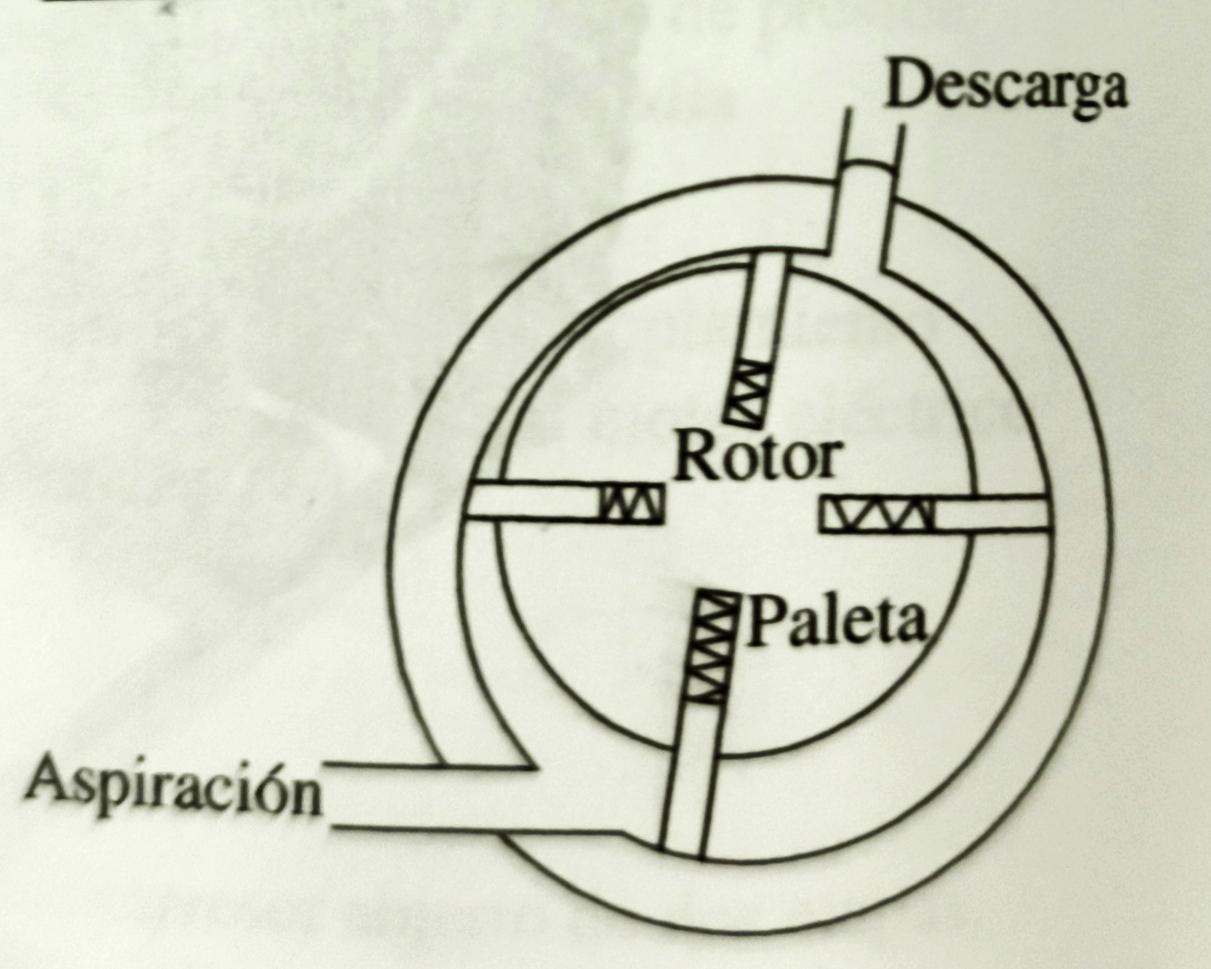
\includegraphics[width=.4\linewidth]{figuras/compresores/rotor de paletas.jpg}
	\caption{Rotor de paletas}
	\label{fig:Rotor de paletas}
\end{figure}

\subsection{Compresores helicoidales}

Los compresores helicoidales o de tornillo son distintos a los anteriormente vistos. La compresi\'on del fluido es continua. Constan de dos rotores llamados primario y secundario que, montados en ambos extremos sobre cojinetes, aseguran su exacta posici\'on en el interior del compresor. El \textbf{rotor primario}, de cuatro l\'obulos o helicoides, es accionado directamente por el motor el\'ectrico y gira a la misma velocidad que \'este.\\ Mediante un sistema de rodamientos, el rotor primario transmite el movimiento al \textbf{rotor secundario}, que tiene seis l\'obulos o helicoides y es del mismo di\'ametro, pero gira a menor velocidad y en sentido contrario.\\ Entre los dos rotores existe una separaci\'on muy pequeña, es decir, no est\'an en contacto entre s\'i.\\Al girar ambos rotores dentro de la cavidad del compresor y debido a esa pequeña separaci\'on, se producen las aberturas de espacios en la zona de aspiraci\'on que con el giro van disminuyendo, con lo que se translada y comprime el fluido hacia el otro extremo de los rotores, donde se produce la descarga del fluido refrigerante.\\ Los hay de tipo herm\'etico, semiherm\'etico y abiertos.
\subsubsection{Importancia del aceite}
Estos compresores helicoidales llevan unos grandes separadores de aceite. Este es inyectado a lo largo de los tornillos para su lubricaci\'on y sellado al mismo tiempo, lo que facilita la compresi\'on del fluido.\\ La \autoref{fig:Circuito de aceite en instalaciones con compresores a tornillo} representa una aplicaci\'on muy utilizada de estos compresores.\\Como consecuencia de la alta temperatura que alcanza el aceite, a la salida del separador y antes de volver al compresor, suele pasar por un enfriador, que seg\'un las caracter\'isticas de la instalaci\'on, puede utilizar aire, agua o el mismo refrigerante para el enfriamiento del aceite.\\ Los factores que determinan si es necesario el enfriamiento del aceite son las condiciones de trabajo:

\begin{itemize}
	\item Temperatura de condensaci\'on
	\item Temperatura de evaporaci\'on
	\item Temperatura de descarga
\end{itemize}

\begin{figure}[H]
	\centering
	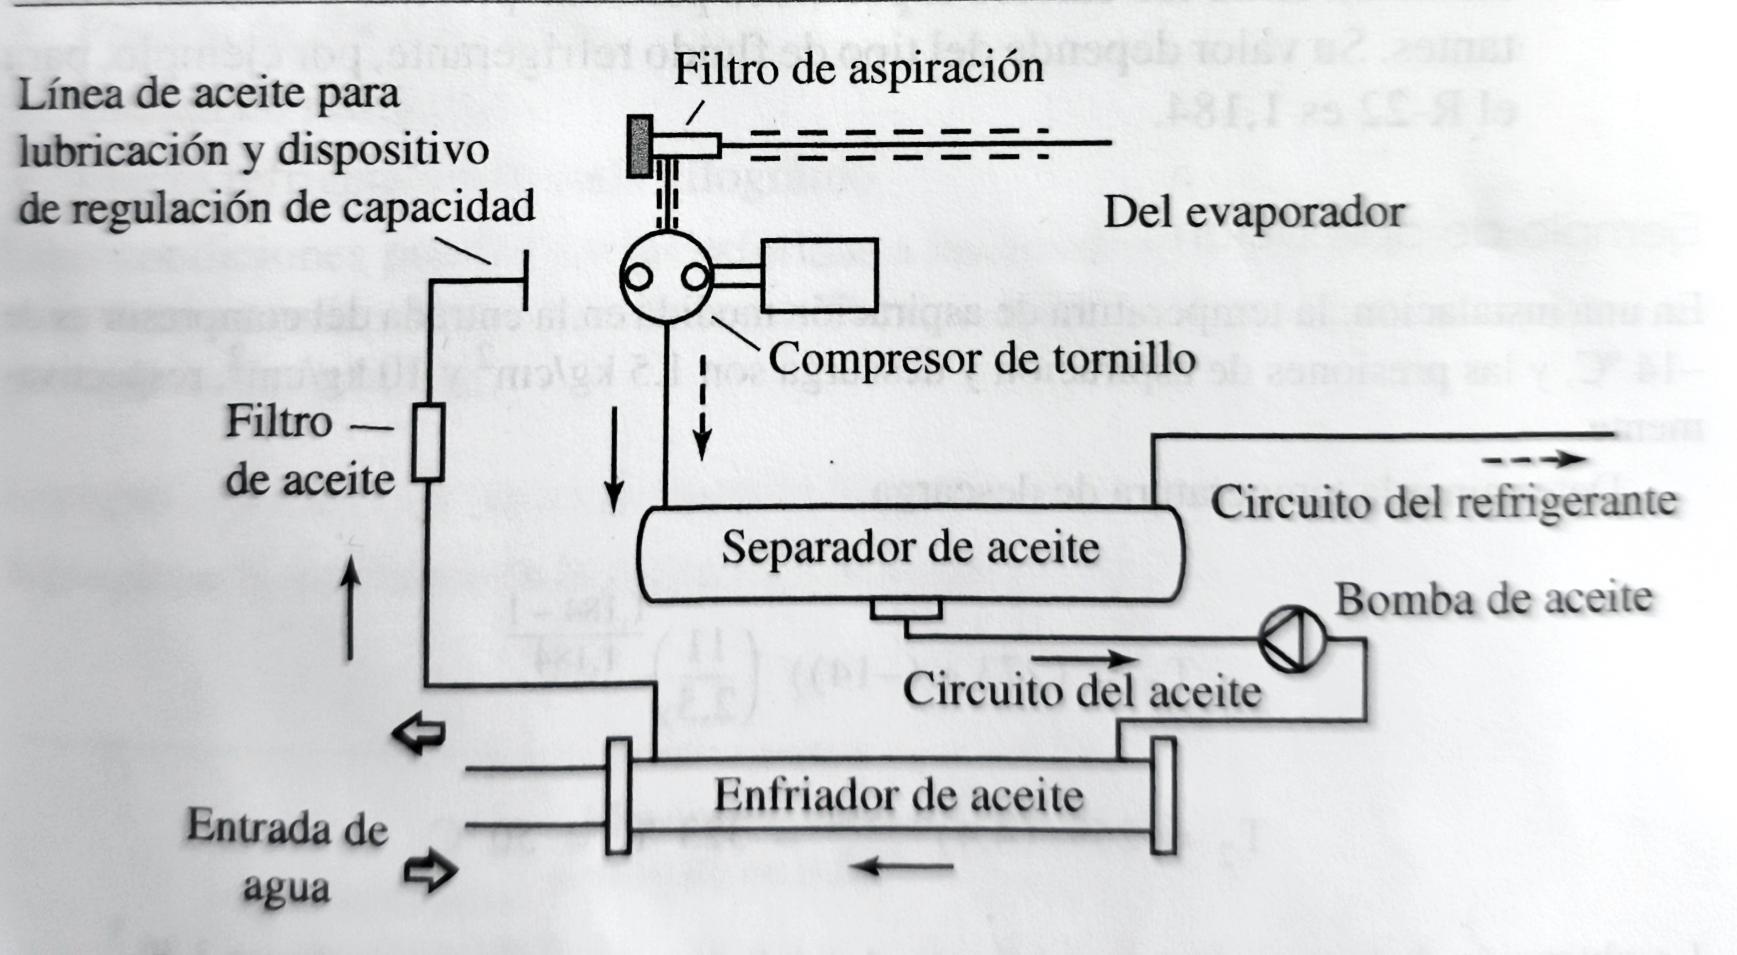
\includegraphics[width=\textwidth]{figuras/compresores/circuito de aceite (2).jpg}
	\caption{Circuito de aceite en instalaciones con compresor a tornillo}
	\label{fig:Circuito de aceite en instalaciones con compresores a tornillo}
\end{figure}

\subsection{Regulación de la potencia}

Si la carga de los evaporadoes siempre fuese la misma, se intalar\'ia el compresor a esa determinada carga t\'ermica. Pero como en la mayor\'ia de los casos la carga var\'ia (ejemplo m\'as notorio lo tenemos en las instalaciones de aire acondicionado), se debe encontrar un punto de equilibrio entre la carga producida por el compresor y la carga necesaria en el evaporador.\\Para los casos de pequeñas instalaciones, como pueden ser heladeras dom\'esticas, el compresor consume muy poca potencia. Por tanto estas instalciones generalmente trabajan con un sistema ON-OFF, donde consumen la potencia m\'axima y una vez que se llego al set point se apaga el compresor.\\En cambop en instalaciones de mayores potencias hay que conseguir un equilibrio entre la carga producida y la necesaria, lo cual significa menores consumos y menos mantenimiento.

\subsubsection{Sistema de regulaci\'on}

La regulaci\'on se puede realizar de varias maneras, por ejemplo actuando sobre el volumen desplazado o bien sobre las revoluciones del motor, ya que la potencia es directamente proporcional a las revoluciones.\\Acontinuaci\'on se presenta un sistema de regulaci\'on para compresores a tornillo:

\begin{enumerate}[a.]
	\item Instalando entre la parte inferior de los rotores y el fondo del c\'arter un dispositivo deslizante (pist\'on), que es accionado por la presi\'on del aceite (mediante electrov\'alvula), y que al desplazarse a lo largo de los rotores, su posici\'on marca el ``punto'' de inicio de la compresi\'on del fluido y determina as\'i el desplazamiento volum\'etrico del compresor.
	\item Mediante controles deslizantes (pistones) instalados en el extremo final de la brida de descarga.
\end{enumerate}

La \autoref{fig:Disposici\'on de los controles de capacidad} representa un compresor semiherm\'etico, en vista superior. La entrada de fluido refrigerante es a trav\'es de la v\'alvula de aspiraci\'on situada en el lado izquierdo, y la descarga (oculta) est\'a en el lado derecho.\\La regulaci\'on de la potencia se realiza mediante las dos electrov\'alvulas y los dos pistones montados en el extremos de la brida de descarga (m\'etodo b.)

\begin{figure}[H]
	\centering
	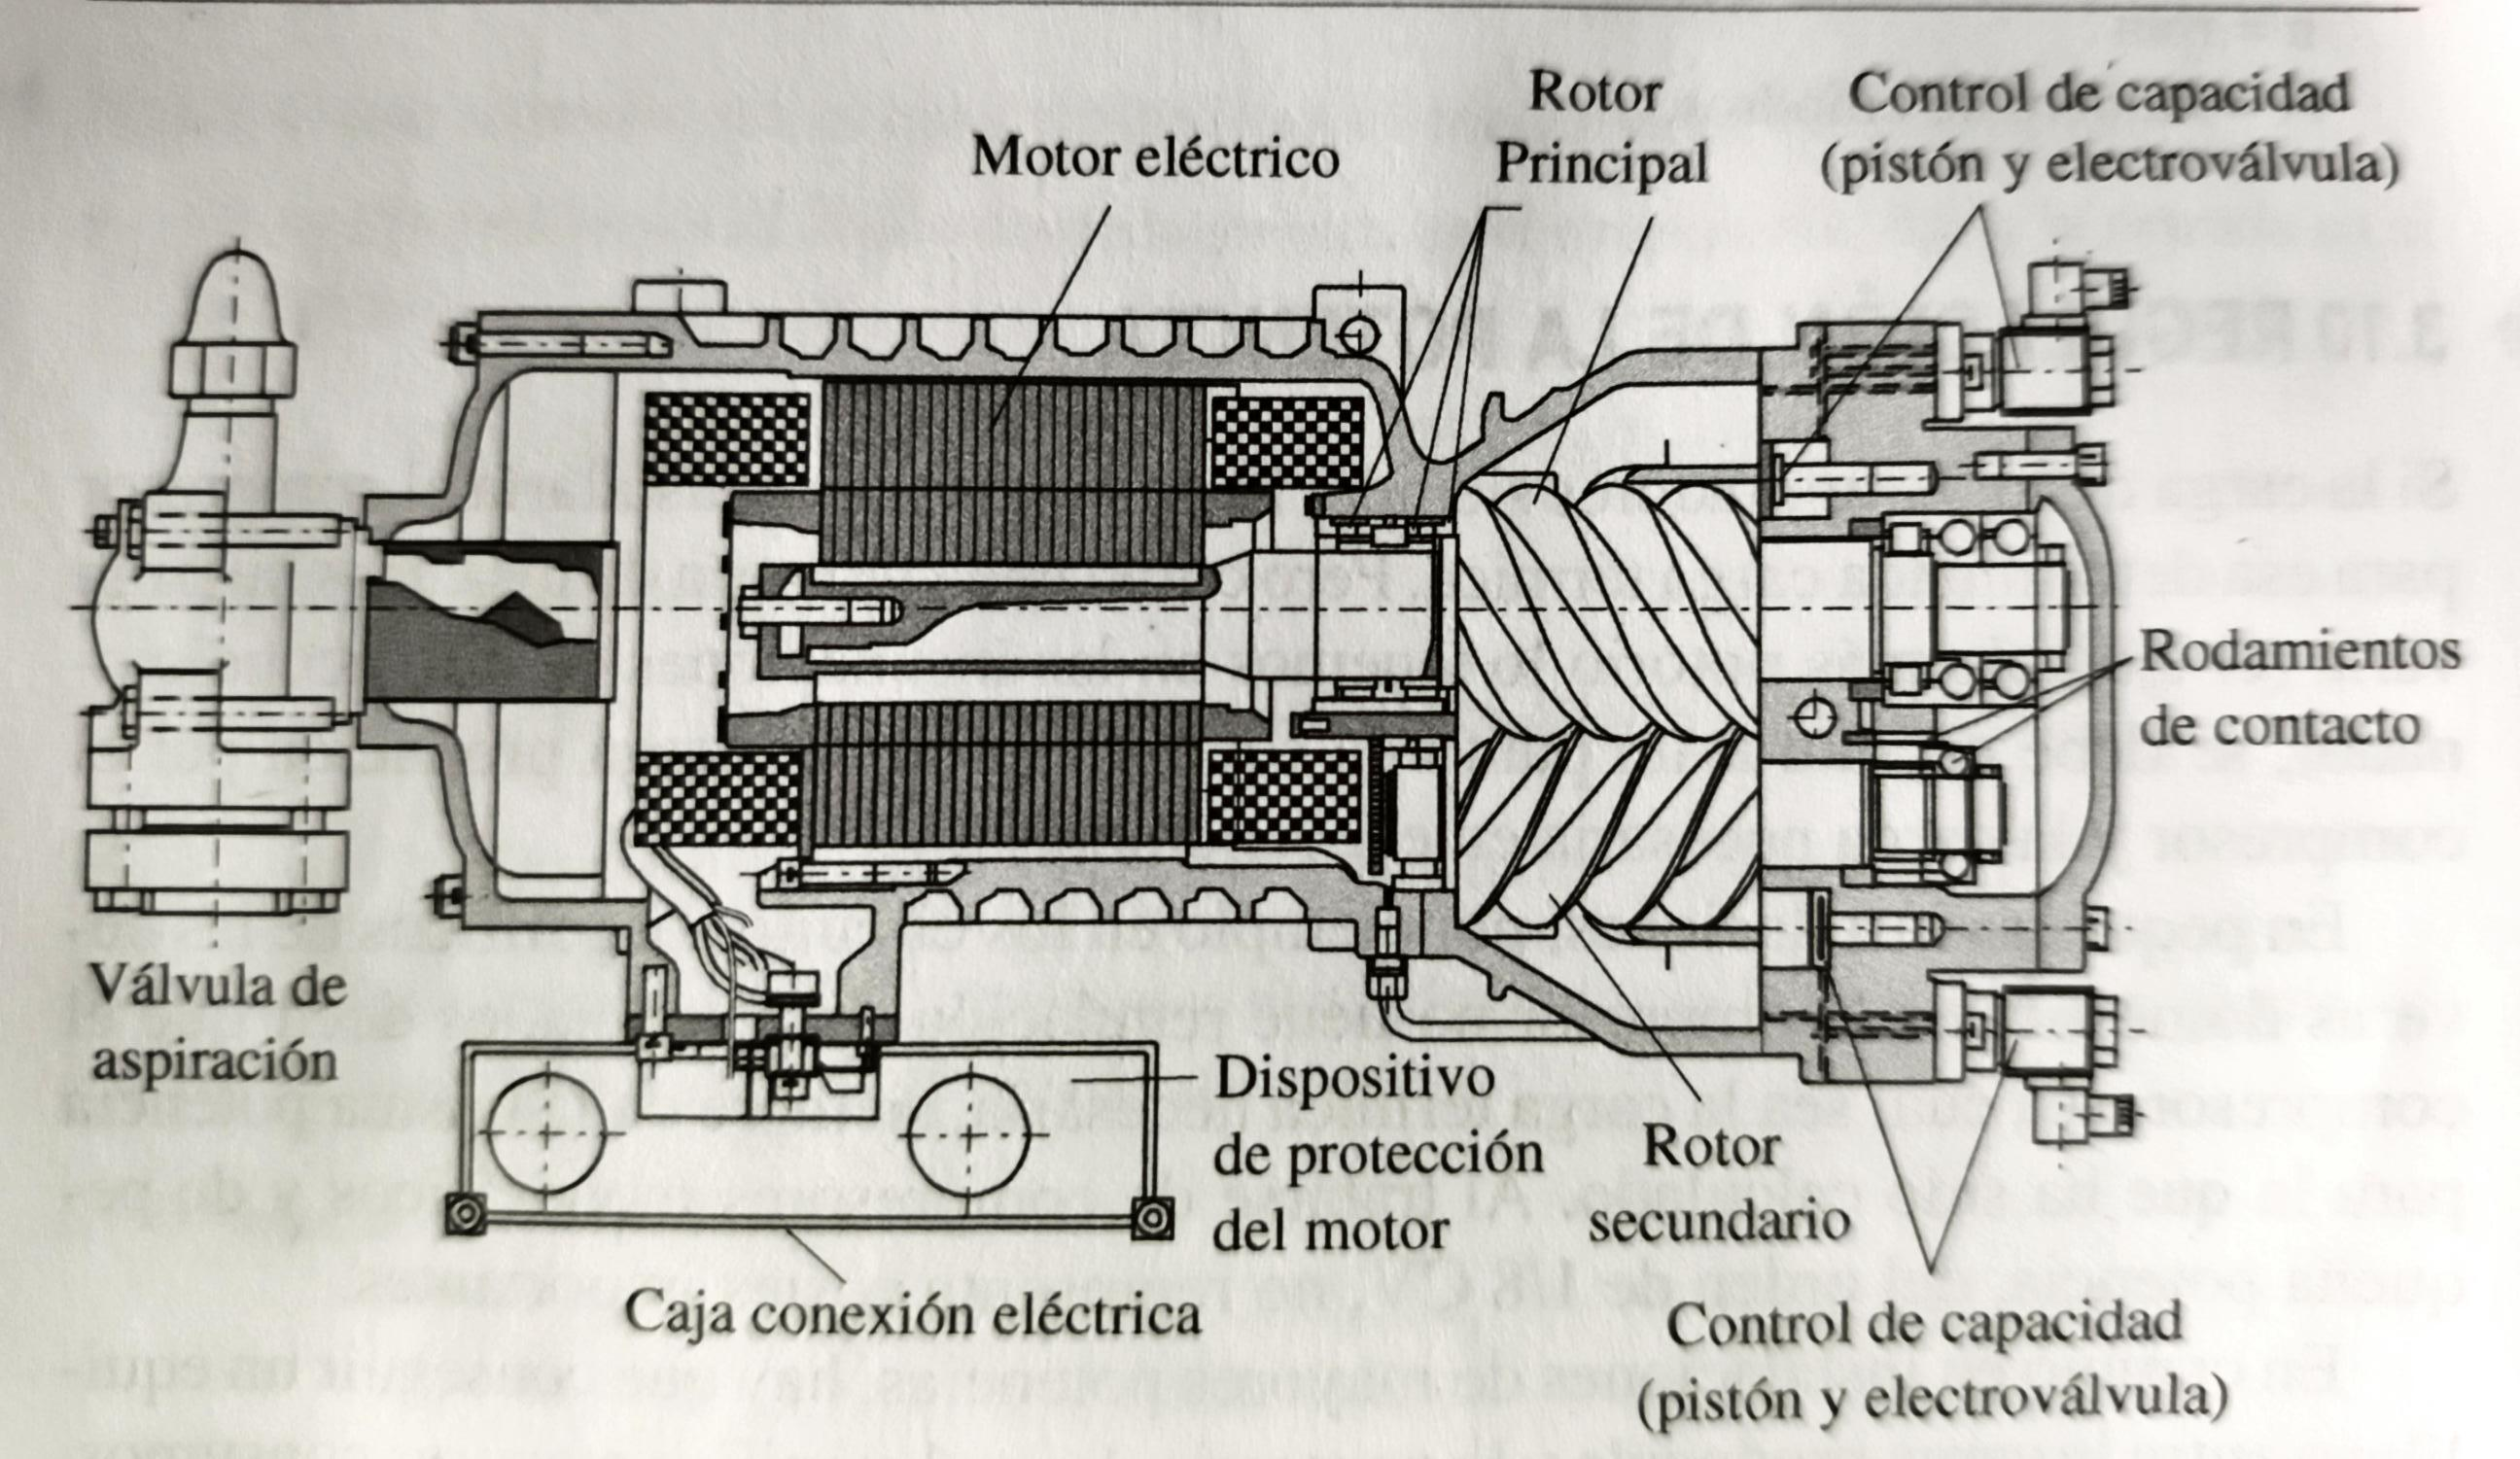
\includegraphics[width=\textwidth]{figuras/compresores/controles de capacidad.jpg}
	\caption{Disposici\'on de los controles de capacidad}
	\label{fig:Disposici\'on de los controles de capacidad}
\end{figure}

\begin{wrapfigure}{r}{0.5\linewidth}
	\centering
	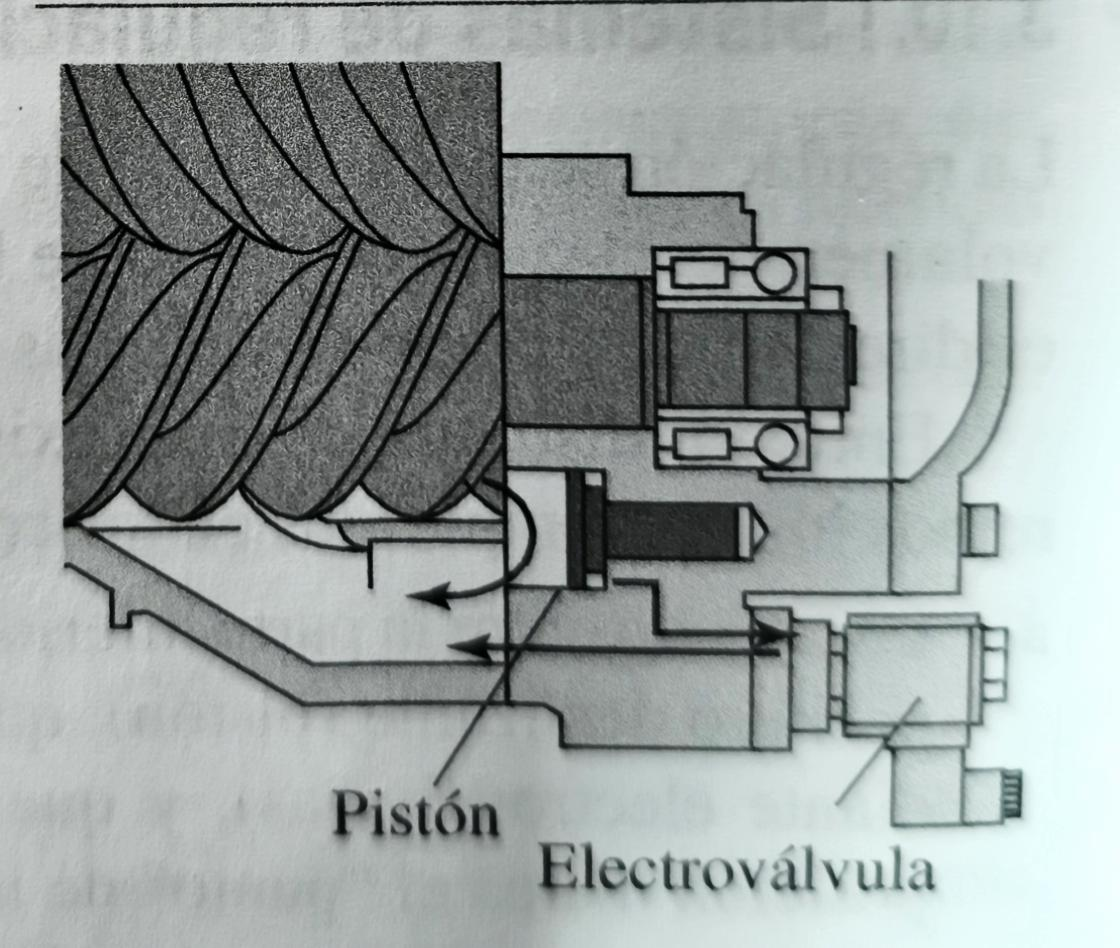
\includegraphics[width=.7\linewidth]{figuras/compresores/detalle de control de capacidad.jpg}
	\caption{Detalle de control de capacidad}
	\label{fig:Detalle de control de capacidad}
\end{wrapfigure}

Los dos pistones son accionados hidr\'aulicamente. Mediante una señal el\'ectrica se abren unos orificios debidamente calibrados, y as\'i una parte del fluido es conducido hacia el lado de la aspiraci\'on (en la \autoref{fig:Detalle de control de capacidad} se aprecia en detalle la operaci\'on)\\Al disminuir el caudal de fluido descargado, tambi\'en se disminuye la potencia. En este sistema, la regulaci\'on de potencia se realiza en dos etapas. Cuando una electrov\'alvula no \'esta activada, se produce una reducci\'on de potencia.

\subsection{Variaciones de las presiones y su repercursión en las potencias}

La potencia frigor\'ifica de un compresor dependen de las condiciones de trabajo. Por ello vamos a ver de que manera repercuten en la potencia frigor\'ifica las variaciones de las presiones de trabajo.\\ En el diagrama de Mollier podemos apreciar c\'omo var\'ia la potencia frigor\'ifica seg\'un las distintas temperaturas de evaporaci\'on y condensaci\'on.
% \renewcommand{\theenumi}{\alph{enumi}}
\begin{enumerate}[a.]
	\item ¿Qu\'e ocurre cuando la presi\'on de aspiraci\'on disminuye?\\ Supongamos que la presi\'on de aspiraci\'on $Pa$, disminuye hasta un valor $Pa^\prime$\\Se comprueba que:
	\begin{enumerate}[1.]
		\item Al disminuir la presi\'on de aspiraci\'on, el efecto refrigerante ($ER^\prime$) tambi\'en disminuye con lo cual disminuye la potencia.
		\item El volumen espec\'ifico ($Ve^\prime$) aumenta, lo que implica que el desplazamiento volum\'etrico disminuye.
	\end{enumerate}

	\begin{figure}[H]
		\centering
		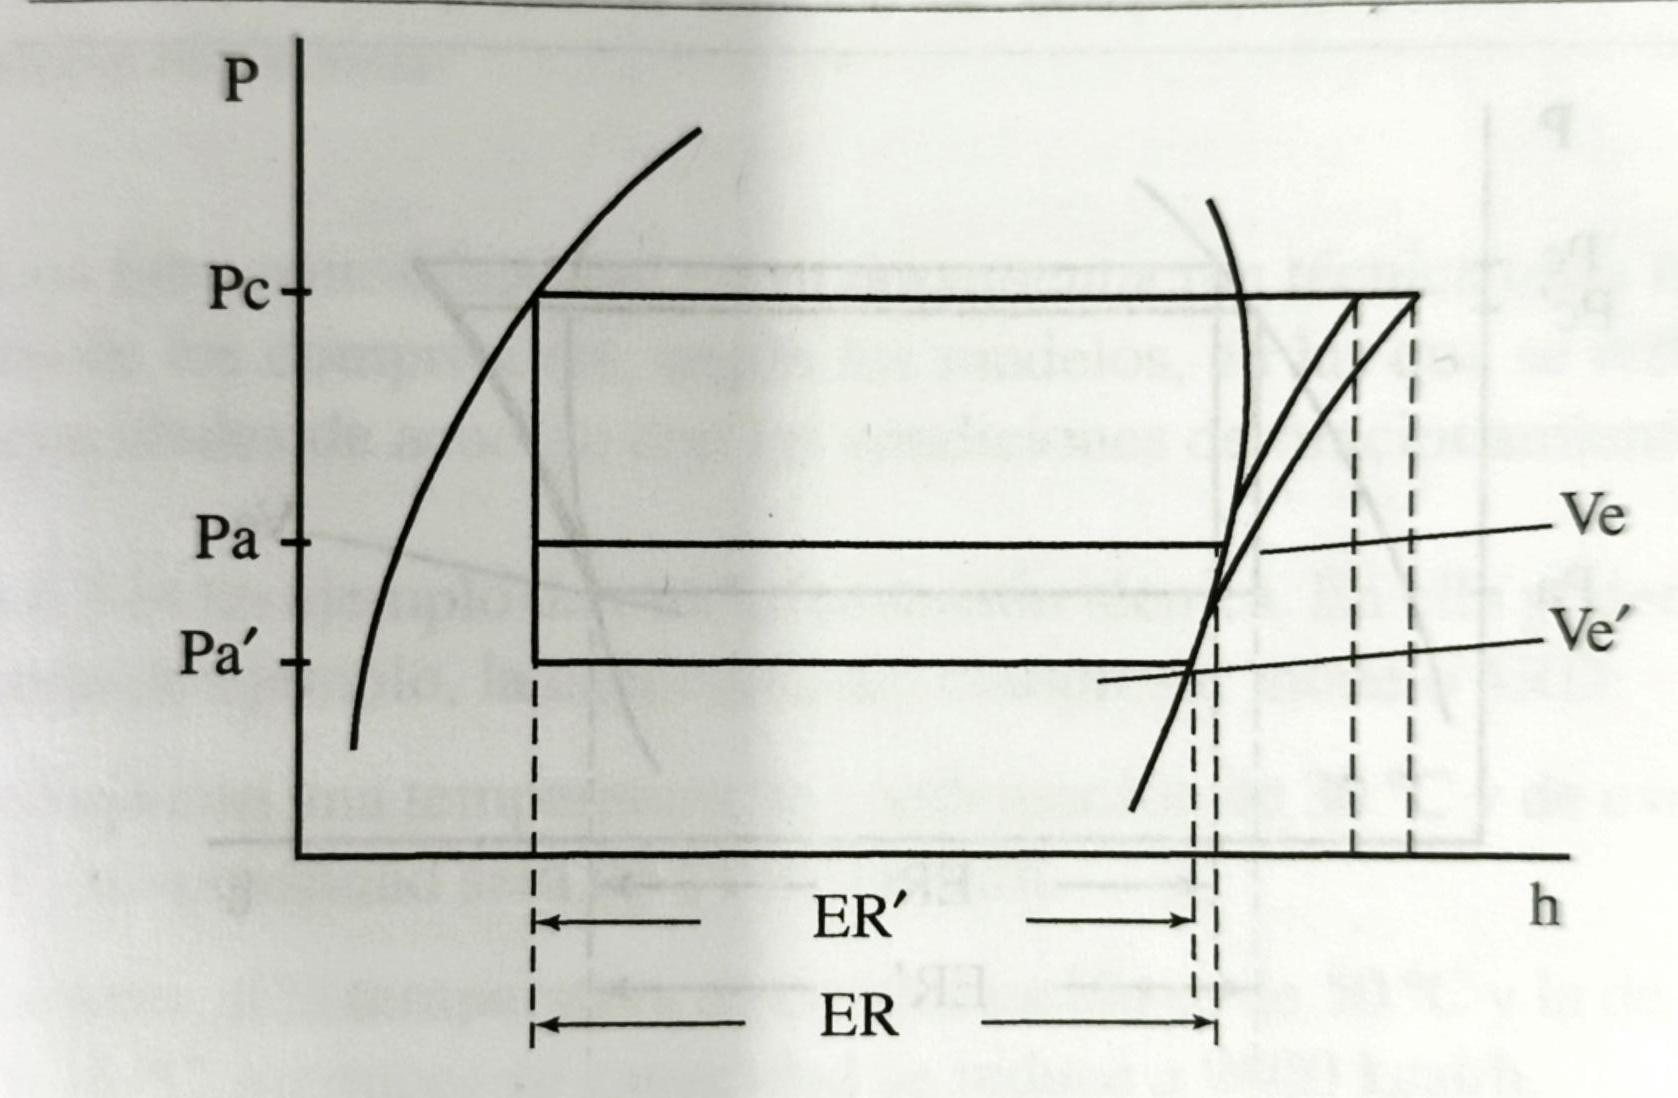
\includegraphics[width=.6\textwidth]{figuras/compresores/variacion de la presion de aspiracion.jpg}
		\caption{Variaci\'on de la psei\'on de aspiraci\'on en el diagrama p-h.}
		\label{Variaci\'on de la presi\'on de aspiraci\'on}
	\end{figure}
	Tambi\'en se puede demostrar num\'ericamente con la relaci\'on de compresi\'on (Rc) para este caso aumenta, por tanto disminuye el rendimiento volum\'etrico (Rv) y la potencia frigor\'ifica.

	\item ¿Qu\'e ocurre con la potencia frigor\'ifica cuando disminuye la presi\'on de condensaci\'on?\\Viendo la \autoref{fig:Variaci\'on de la presi\'on de condensaci\'on} se puede ver que:
	\begin{enumerate}[1.]
		\item El efecto refrigerante ($ER^\prime$) aumenta, con lo que la potencia frigor\'ifica tambi\'en aumenta.
		\item La relaci\'on de compresi\'on (Rc) disminuye, con lo que la potencia frigor\'ifica aumenta.
	\end{enumerate}
	\begin{figure}[H]
		\centering
		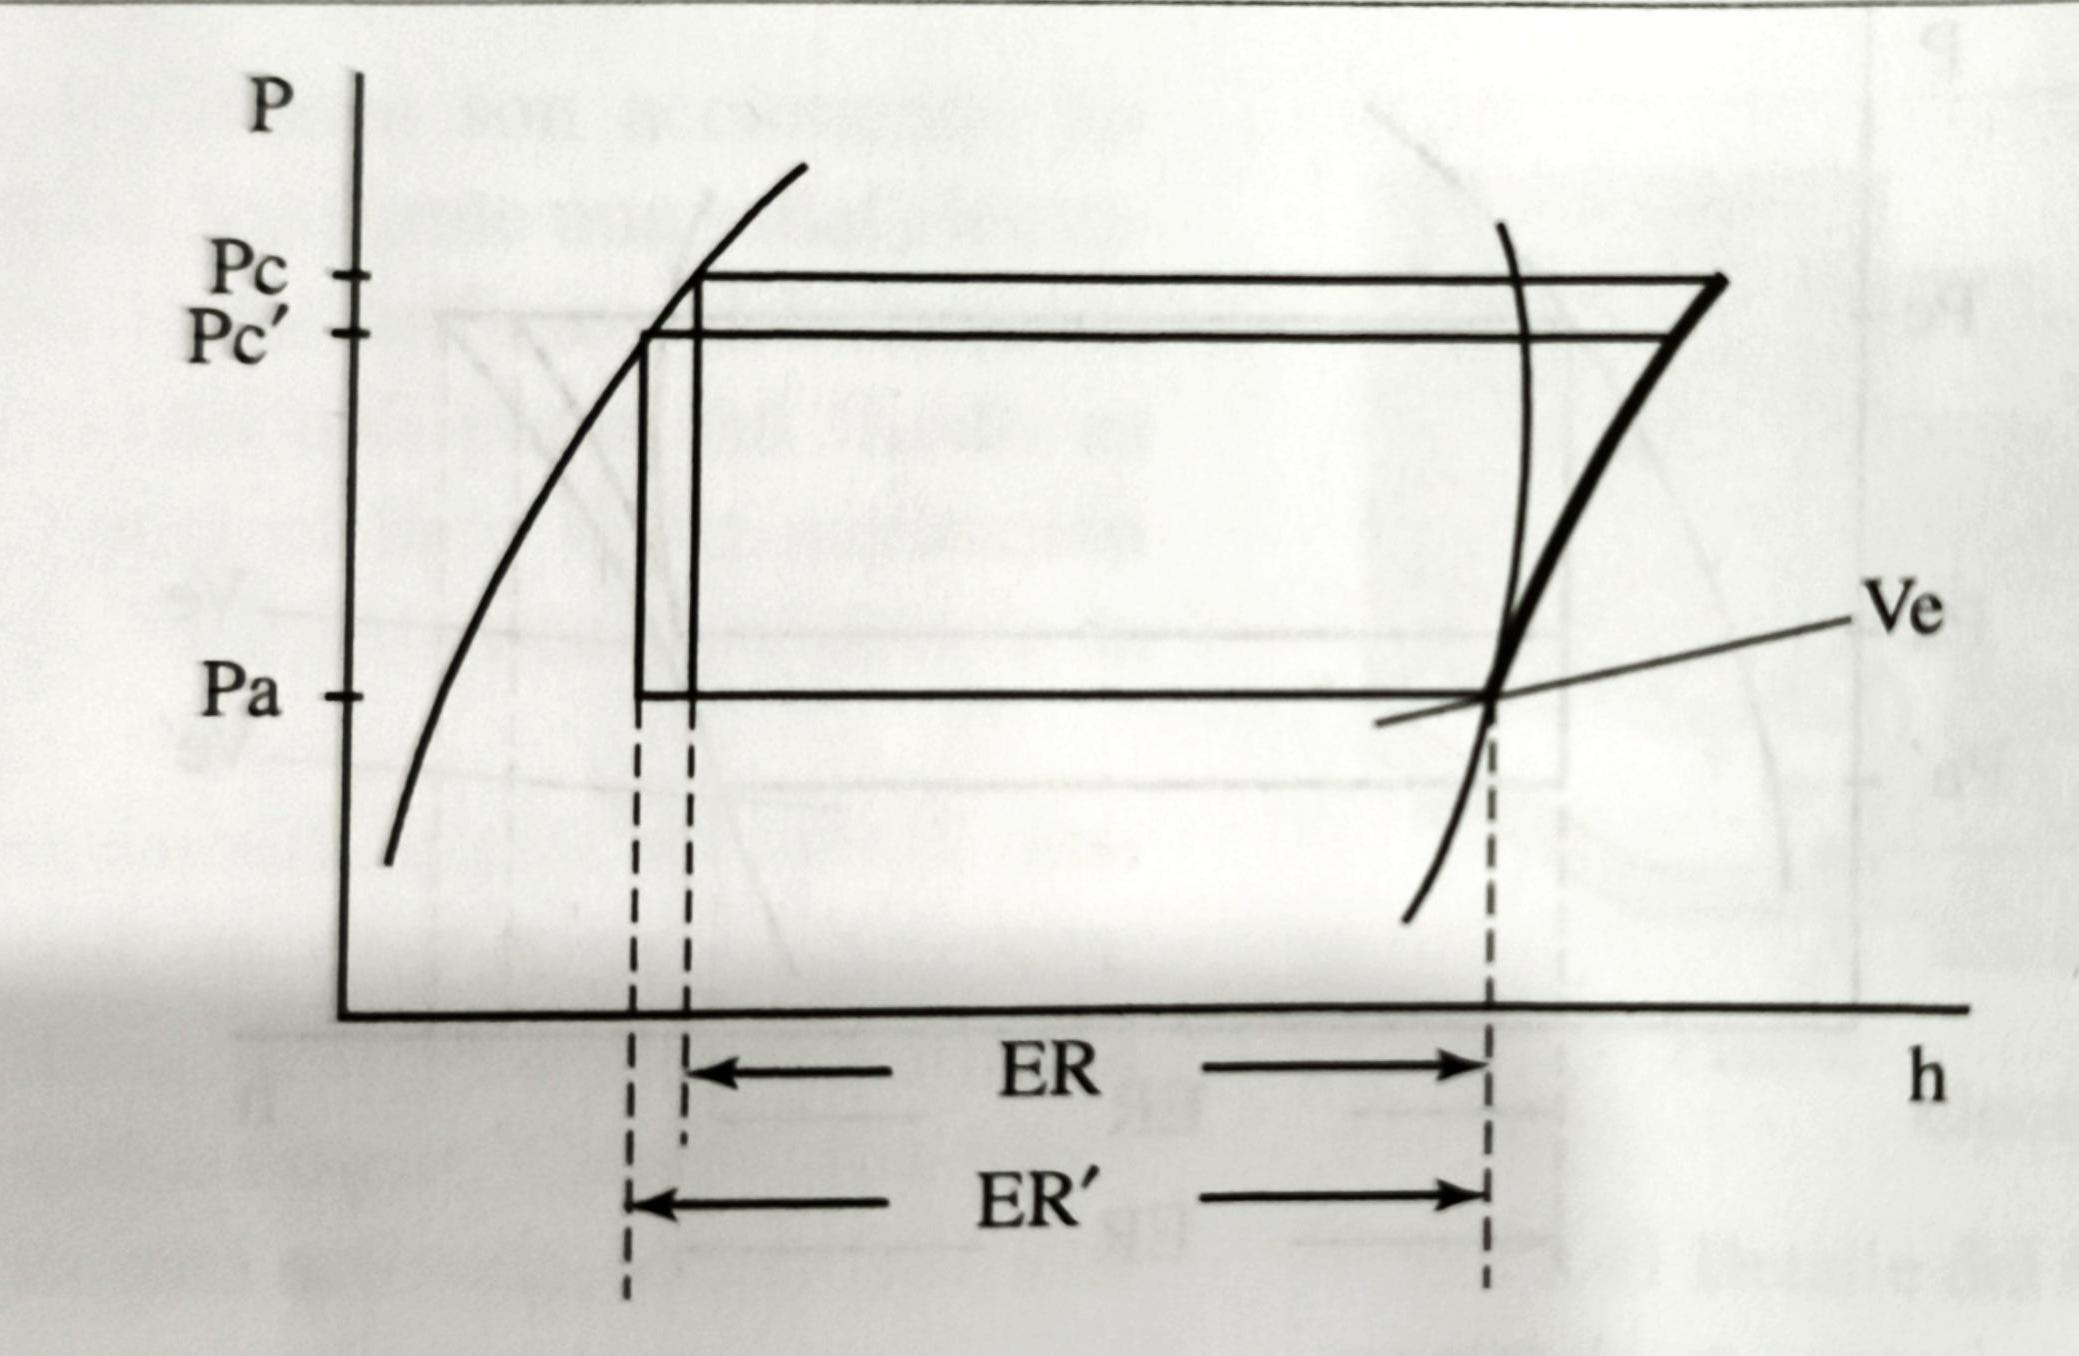
\includegraphics[width=.6\textwidth]{figuras/compresores/variacion de la presion de condensacion.jpg}
		\caption{Variaci\'on de la presi\'on de condensaci\'on en el diagrama p-h}
		\label{fig:Variaci\'on de la presi\'on de condensaci\'on}
	\end{figure}
\end{enumerate}
La \autoref{fig:Capacidad de un compresor modelo 4RD} es un ejemplo es informaci\'on t\'ecnica de un compresor modelo 4RD, en ella podemos corroborar lo anteriormente dicho:
\begin{enumerate}[a.]
	\item Si la temperatura de condensaci\'on es 30\textcelsius\ y de evaporaci\'on -5\textcelsius, entonces su capacidad ser\'a de 11800 kcal/h.
	\item En cambio, si la temperatura de condensaci\'on es de 50\textcelsius\ y la de evaporaci\'on es de -5\textcelsius, entonces su capacidad se reduce a 9400 kcal/h.
\end{enumerate}
\begin{figure}[h]
	\centering
	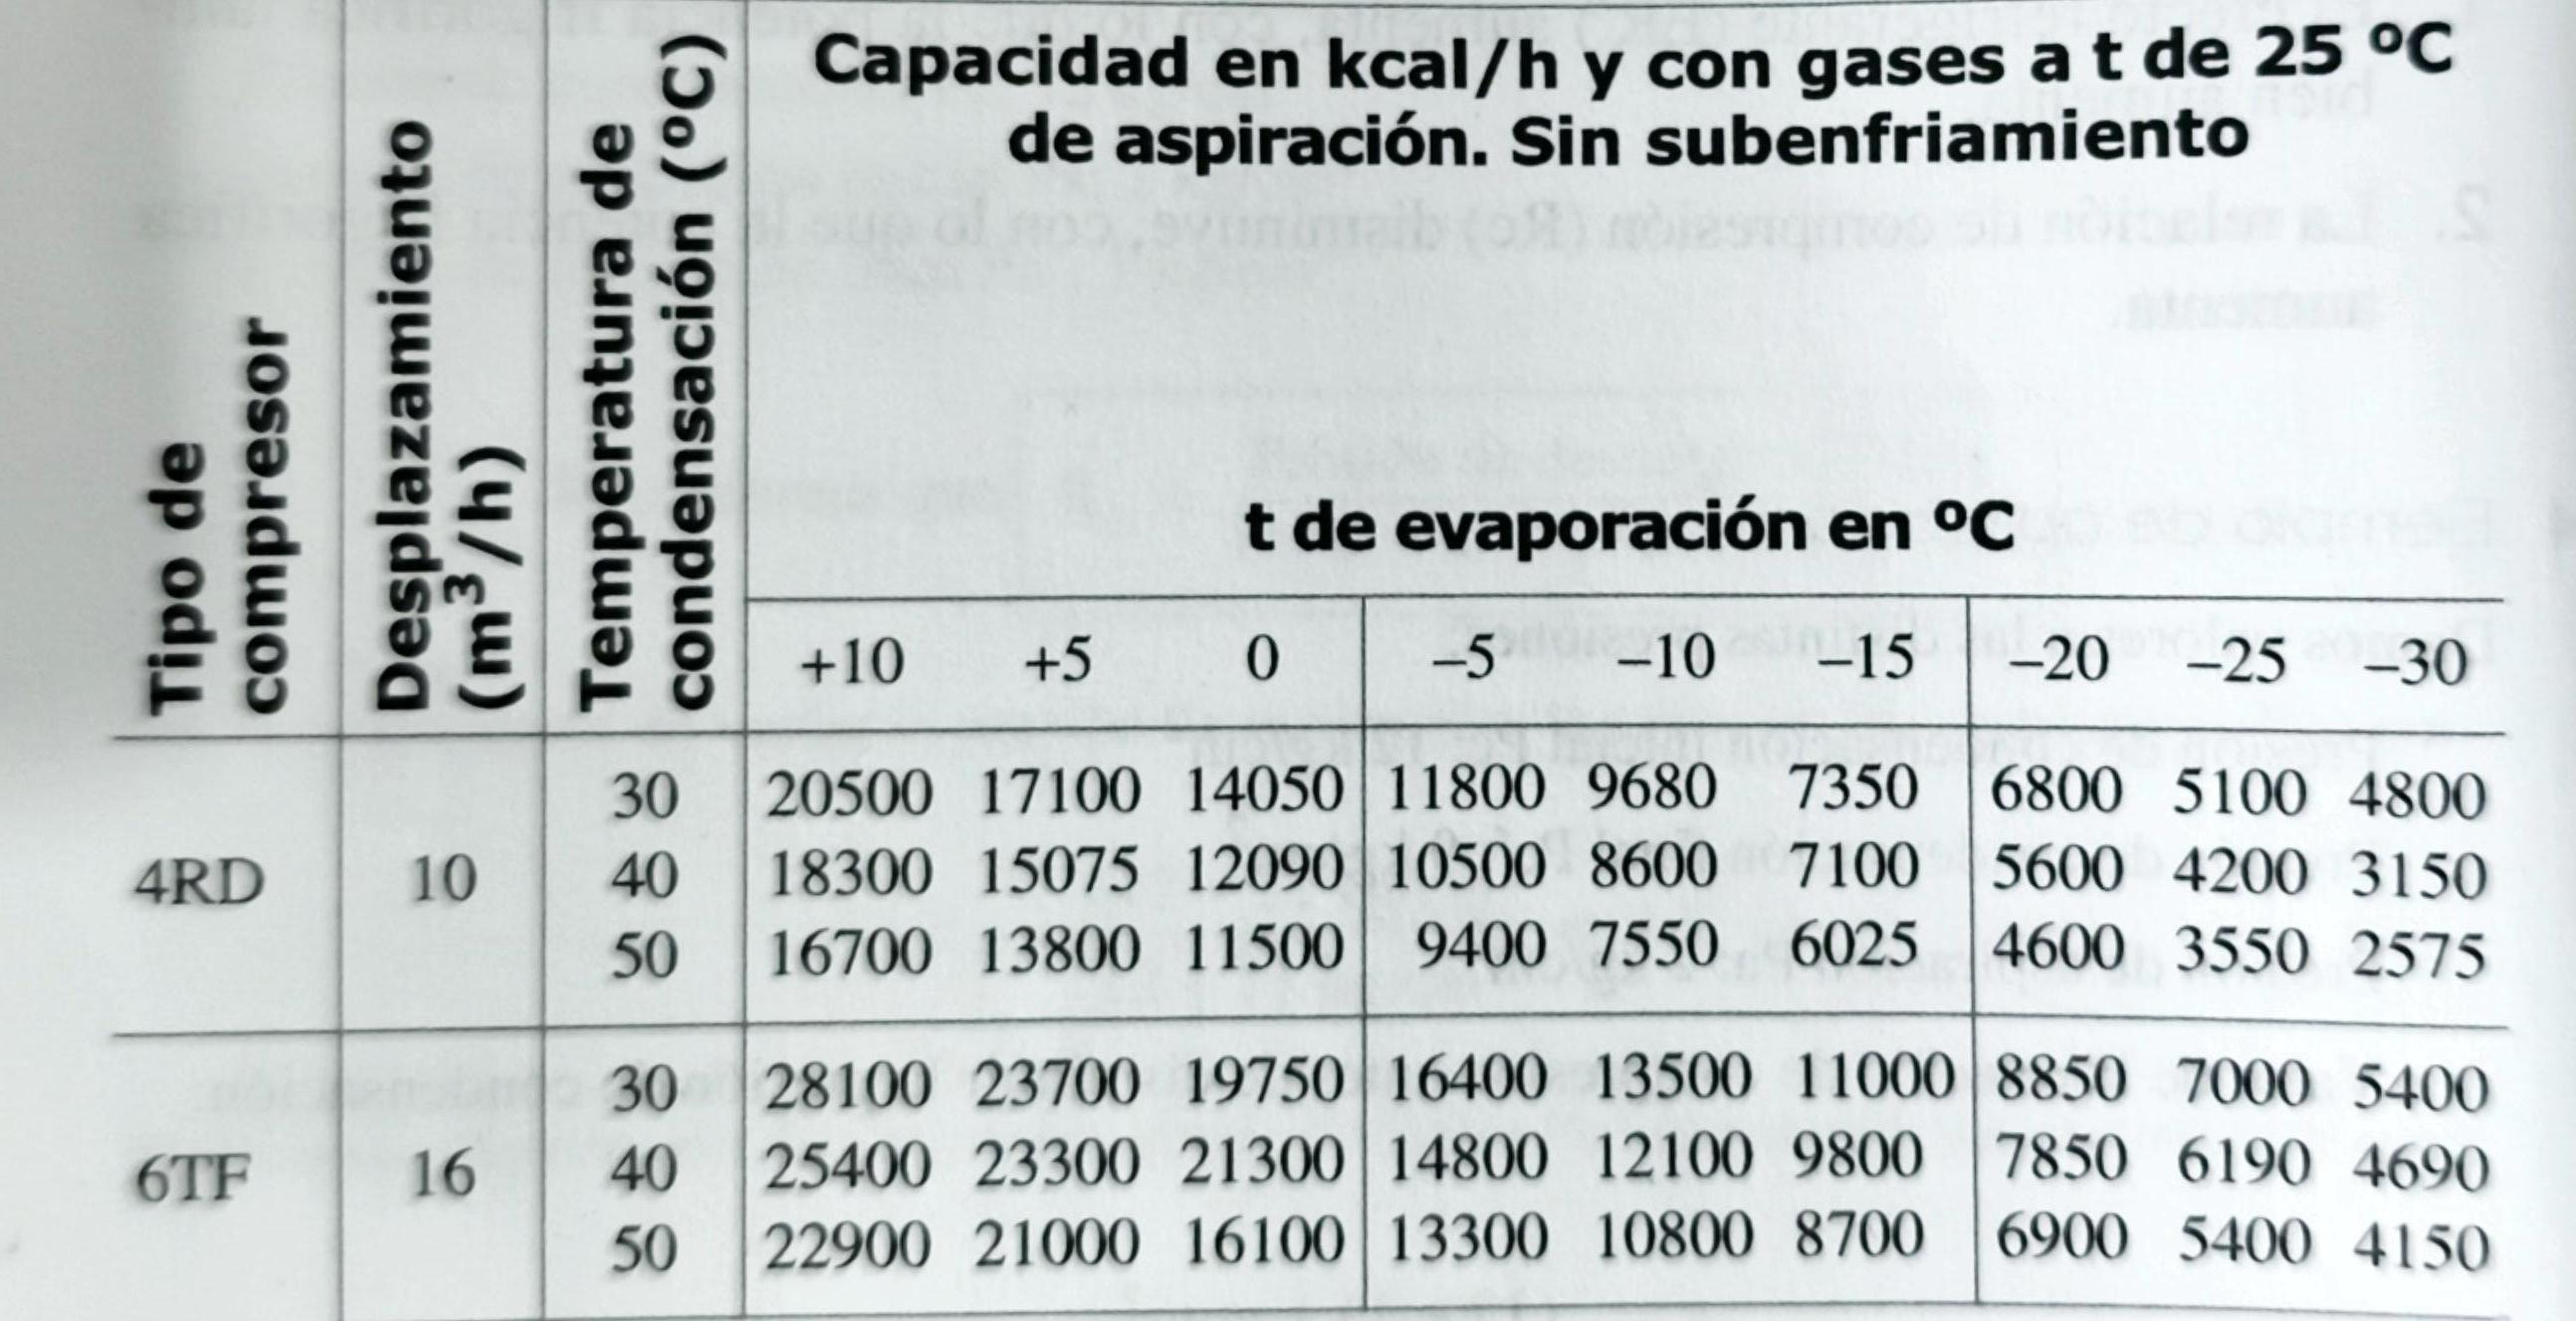
\includegraphics[width=\linewidth]{figuras/compresores/tabla de capacidad de un compresor.jpg}
	\caption{Capacidad de un compresor modelo 4RD}
	\label{fig:Capacidad de un compresor modelo 4RD}
\end{figure}
\subsection{Funcionamiento en régimen seco y en régimen húmedo}
Se dice que trabaja en \textsl{r\'egimen h\'umedo} cuando el fluido a la entrada del compresor es una mezcla de gas y l\'iquido (Tramo 1-2 de la \autoref{fig:R\'egimen seco y h\'umedo}). Esto puede ocurrir por diversas causas, tales como:
\begin{enumerate}[a.]
	\item Mala regulaci\'on del dispositivo de expansi\'on y entra demasiado fluido refrigerante en el evaporador.
	\item Mala circulaci\'on del aire a trav\'es del evaporador por obstrucci\'on o por caudal insuficiente.
\end{enumerate}
Pero en esa mezcla, la cantidad de l\'iquido a\'un no es lo suficiente importante para producir el golpe de l\'iquido, ya que se va evaporando debido a las temperaturas m\'as altas que se va encontrando, por ejemplo:
\begin{enumerate}[a.]
	\item En la conexi\'on tuber\'ia de aspiraci\'on-compresor
	\item En la culata
	\item En el pist\'on
	\item En la camisa
	\item Durante la fase de compresi\'on 
\end{enumerate}

\begin{wrapfigure}{r}{0.5\linewidth}
	\centering
	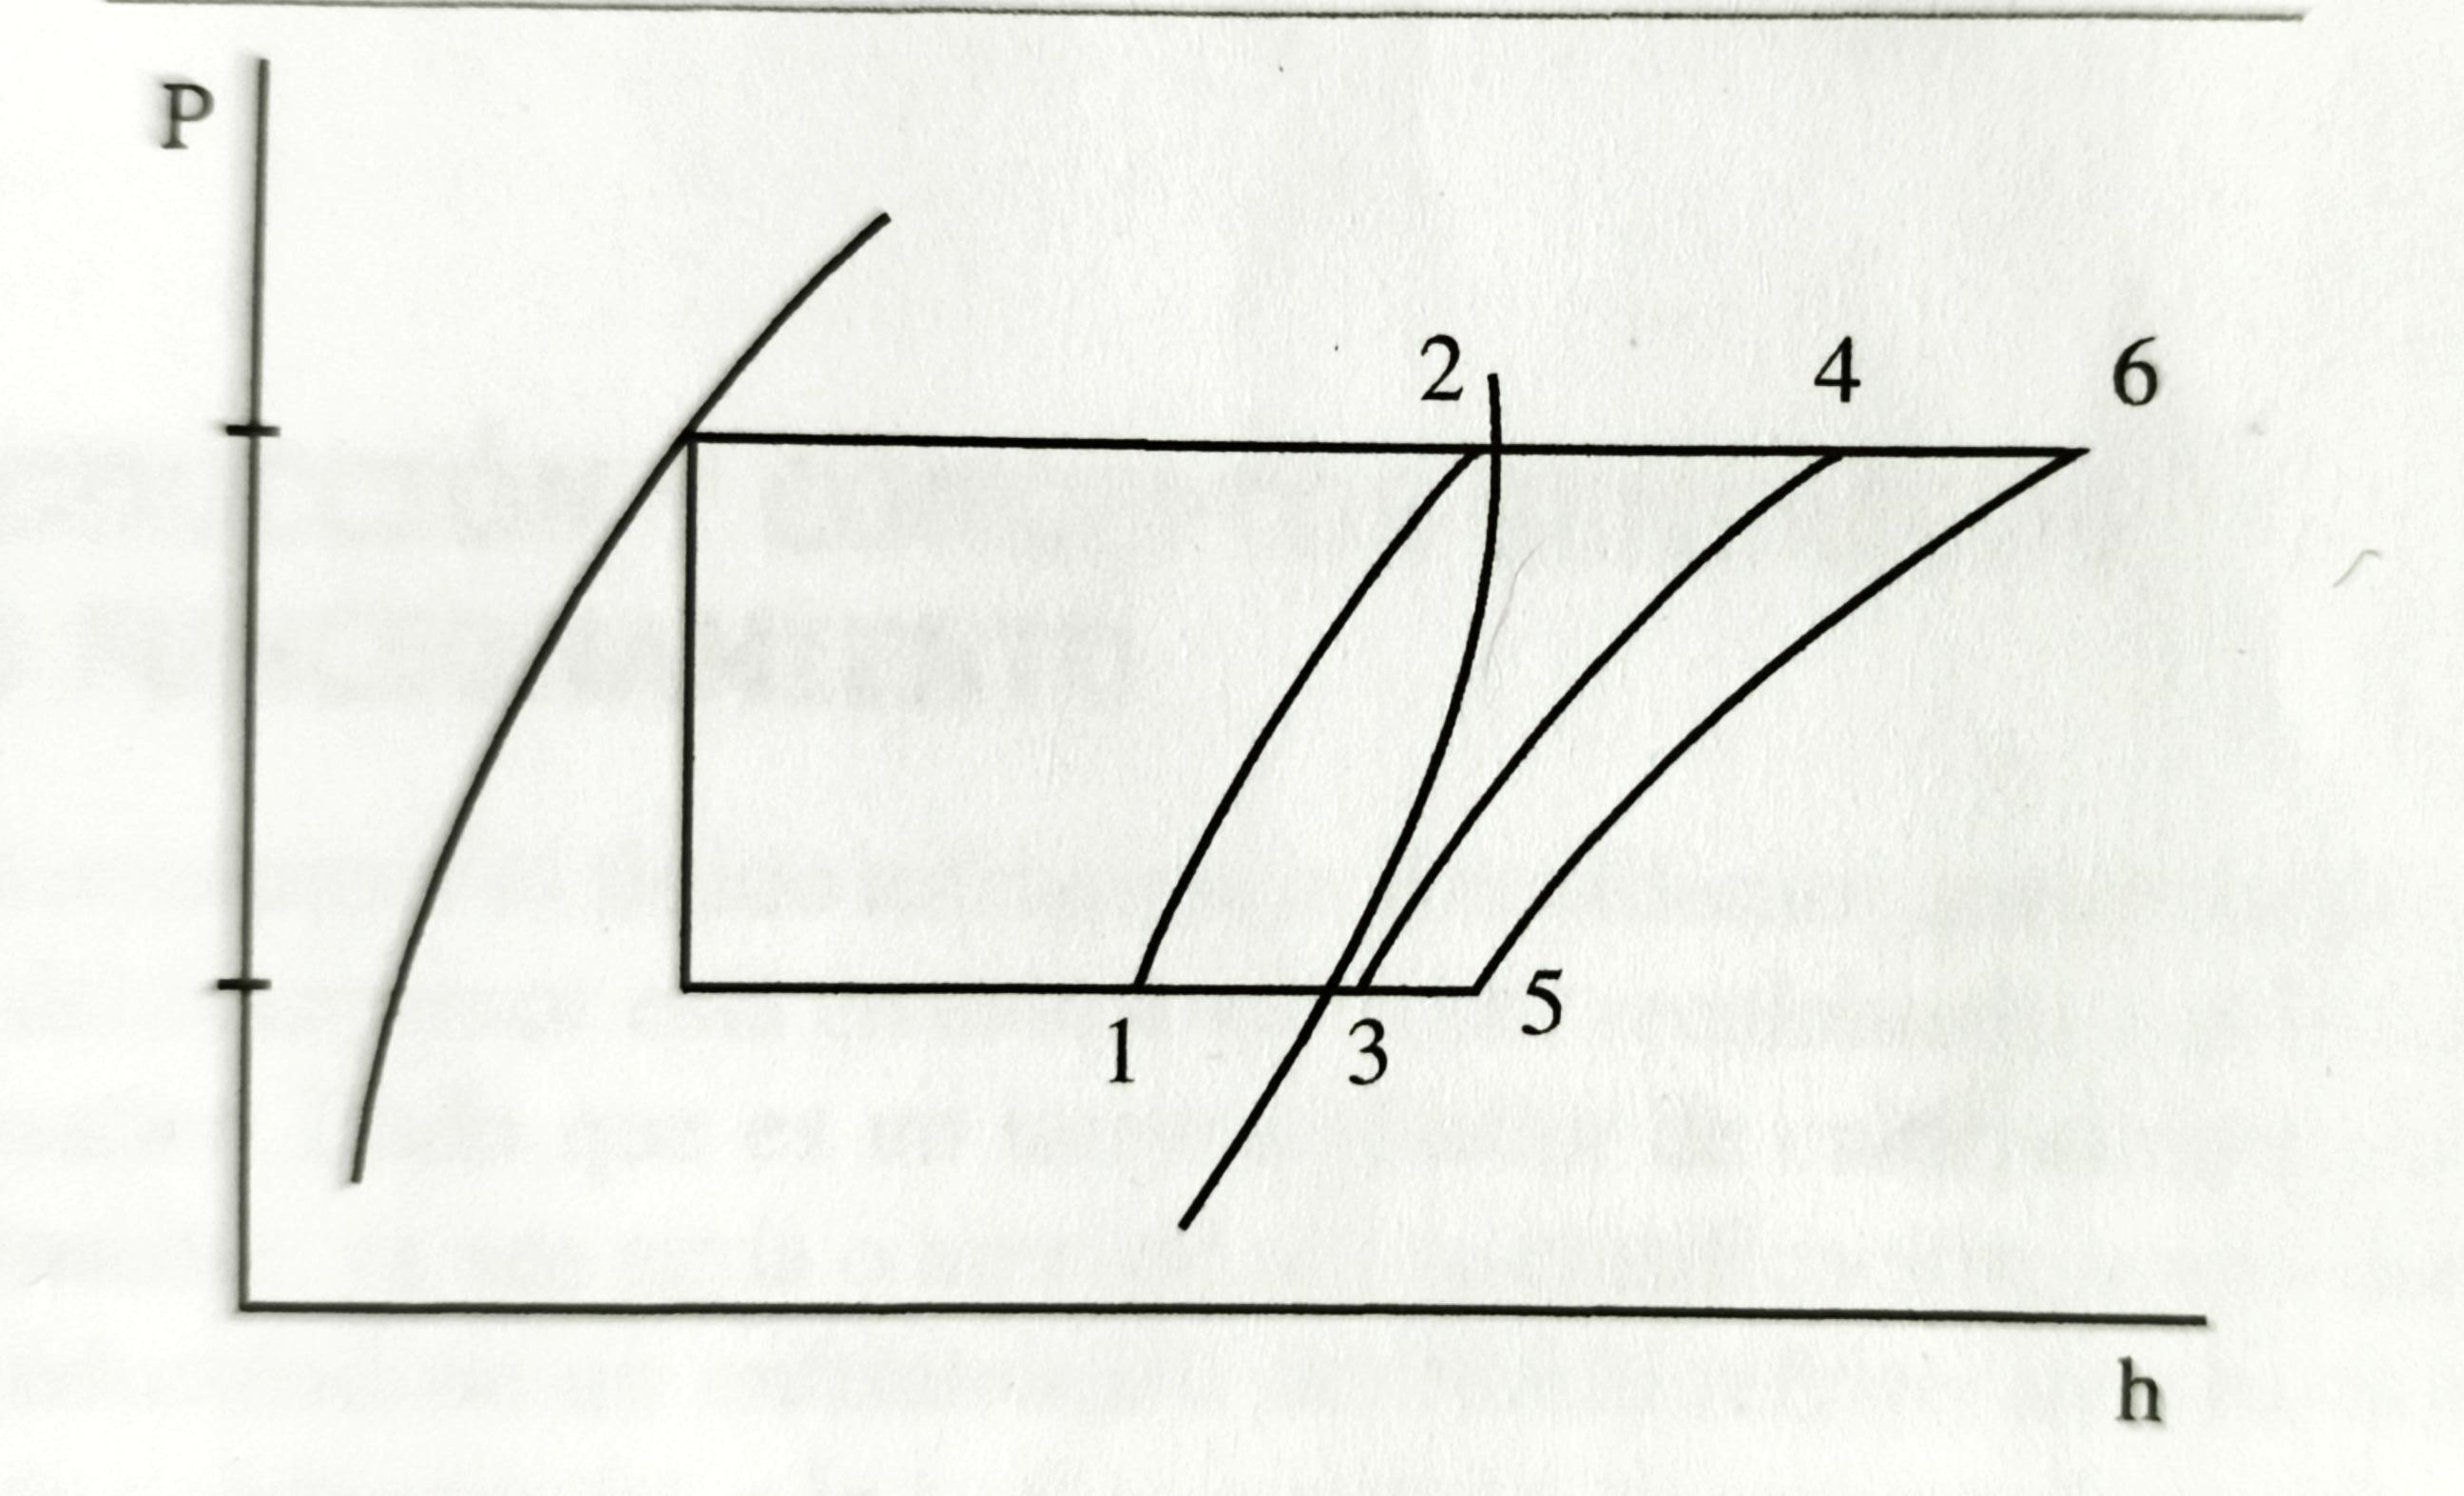
\includegraphics[width=.8\linewidth]{figuras/compresores/régimen seco y humedo.jpg}
	\caption{R\'egimen seco y h\'umedo}
	\label{fig:R\'egimen seco y h\'umedo}
\end{wrapfigure}

Pero ese calor que absorbe el l\'iquido lo est\'a haciendo del calor proveniente del compresor e instalaci\'on y no del ambiente a refrigerar (en el evaporador).\\ En cambio, cuando el fluido a la entrada del compresor es vapor (Tramo 3-4 de la \autoref{fig:R\'egimen seco y h\'umedo}), entonces se trata del \textbf{r\'egimen seco} y, en este caso, el rendimiento es mayor que en el caso anterior. Pero se debe tener especial cuidado para este tipo de funcionamiento, ya que si el vapor que entra al compresor est\'a demasiado sobrecalentado puede generar temperaturas de descarga elevadas por lo que el rendimiento del ciclo ser\'a perjudicado (Tramo 5-6 de la \autoref{fig:R\'egimen seco y h\'umedo}).		

